% !TeX program = xelatex
% !TeX encoding = UTF-8
% 编译方法：在本目录下执行 xelatex main.tex（建议连续编译两次以更新交叉引用）
% 编译前请确认 figures/ 下的图件已按 figures/README.md 的来源说明放置。
\documentclass[UTF8,a4paper,zihao=-4,fontset=none]{ctexart}

% 字体采用三级自动选择机制，使模板能够在不同电脑上直接编译。
% 先检查 Windows 标准字体目录；再检查 macOS 版 Microsoft Word 的字体；均不可用时回退到 TeX Live 自带的 Fandol 字体。
% 无论选择哪一组字体，主字体的 BoldFont 都显式绑定到对应黑体，确保 \textbf 下的中文字体正确。
\newcommand{\UseWindowsMicrosoftFonts}{
  \setCJKmainfont{simsun.ttc}[Path={C:/Windows/Fonts/},BoldFont=simhei.ttf]
  \setCJKsansfont{simhei.ttf}[Path={C:/Windows/Fonts/},BoldFont=simhei.ttf]
  \setCJKmonofont{simsun.ttc}[Path={C:/Windows/Fonts/}]
  \setCJKfamilyfont{paperhei}{simhei.ttf}[Path={C:/Windows/Fonts/},BoldFont=simhei.ttf]
  \PackageInfo{paper-template}{Using Windows SimSun and SimHei}
}

\newcommand{\UseOfficeMicrosoftFonts}{
  \setCJKmainfont{Simsun.ttc}[
    Path={/Applications/Microsoft Word.app/Contents/Resources/DFonts/},
    BoldFont=SimHei.ttf
  ]
  \setCJKsansfont{SimHei.ttf}[
    Path={/Applications/Microsoft Word.app/Contents/Resources/DFonts/},
    BoldFont=SimHei.ttf
  ]
  \setCJKmonofont{Simsun.ttc}[
    Path={/Applications/Microsoft Word.app/Contents/Resources/DFonts/}
  ]
  \setCJKfamilyfont{paperhei}{SimHei.ttf}[
    Path={/Applications/Microsoft Word.app/Contents/Resources/DFonts/},
    BoldFont=SimHei.ttf
  ]
  \PackageInfo{paper-template}{Using Microsoft Office SimSun and SimHei}
}

\newcommand{\UsePortableFandolFonts}{
  \setCJKmainfont{FandolSong-Regular.otf}[cmap=UniGB-UTF16-H,BoldFont=FandolHei-Regular.otf]
  \setCJKsansfont{FandolHei-Regular.otf}[cmap=UniGB-UTF16-H,BoldFont=FandolHei-Regular.otf]
  \setCJKmonofont{FandolFang-Regular.otf}[cmap=UniGB-UTF16-H]
  \setCJKfamilyfont{paperhei}{FandolHei-Regular.otf}[cmap=UniGB-UTF16-H,BoldFont=FandolHei-Regular.otf]
  \PackageWarningNoLine{paper-template}{SimSun and SimHei not found; using portable Fandol fonts}
}

\newcommand{\UseOfficeOrPortableFonts}{
  \IfFileExists{/Applications/Microsoft Word.app/Contents/Resources/DFonts/Simsun.ttc}{
    \IfFileExists{/Applications/Microsoft Word.app/Contents/Resources/DFonts/SimHei.ttf}{
      \UseOfficeMicrosoftFonts
    }{
      \UsePortableFandolFonts
    }
  }{
    \UsePortableFandolFonts
  }
}

% 将下面的 0 改为 1，可强制使用完全随 TeX Live 提供的 Fandol 字体进行兼容性测试。
\providecommand{\ForcePortableFonts}{0}
\ifnum\ForcePortableFonts=1
  \UsePortableFandolFonts
\else
  \IfFileExists{C:/Windows/Fonts/simsun.ttc}{
    \IfFileExists{C:/Windows/Fonts/simhei.ttf}{
      \UseWindowsMicrosoftFonts
    }{
      \UseOfficeOrPortableFonts
    }
  }{
    \UseOfficeOrPortableFonts
  }
\fi
\newcommand{\heifont}{\CJKfamily{paperhei}}

% 页面、行距与段落。
\usepackage[a4paper,top=2.5cm,bottom=2.5cm,left=2.5cm,right=2.5cm,footskip=1.2cm]{geometry}
\usepackage{setspace}
\singlespacing
\setlength{\parindent}{2em}
\setlength{\parskip}{0pt}

% 数学公式、表格与插图。
\usepackage{amsmath,amssymb,mathtools,bm}
\usepackage{graphicx}
\usepackage{booktabs,tabularx,array,multirow}
\usepackage[table]{xcolor}
\usepackage{float}
\usepackage{caption}
\usepackage{subcaption}
\usepackage{enumitem}
\graphicspath{{figures/}}

% 标题、页码与交叉引用。
\usepackage{titlesec}
\usepackage{fancyhdr}
\usepackage[hidelinks]{hyperref}
\usepackage{cleveref}

% 一级标题使用中文序号并居中，下级标题使用阿拉伯数字层级编号并左对齐。
\renewcommand{\thesection}{\arabic{section}}
\renewcommand{\thesubsection}{\arabic{section}.\arabic{subsection}}
\renewcommand{\thesubsubsection}{\arabic{section}.\arabic{subsection}.\arabic{subsubsection}}
\setcounter{secnumdepth}{3}
\titleformat{\section}[block]
  {\centering\heifont\bfseries\zihao{4}}
  {\chinese{section}、}{0pt}{}
\titleformat{\subsection}[hang]
  {\raggedright\heifont\bfseries\zihao{-4}}
  {\thesubsection}{0.8em}{}
\titleformat{\subsubsection}[hang]
  {\raggedright\heifont\bfseries\zihao{-4}}
  {\thesubsubsection}{0.8em}{}
\titlespacing*{\section}{0pt}{2.8ex plus 0.5ex minus 0.2ex}{1.7ex}
\titlespacing*{\subsection}{0pt}{1.6ex plus 0.3ex minus 0.1ex}{0.8ex}
\titlespacing*{\subsubsection}{0pt}{1.4ex plus 0.2ex minus 0.1ex}{0.7ex}

% 页码从摘要页开始，位于页脚中央。
\pagestyle{fancy}
\fancyhf{}
\fancyfoot[C]{\zihao{5}\thepage}
\renewcommand{\headrulewidth}{0pt}
\renewcommand{\footrulewidth}{0pt}

% 图表及列表的常用设置。
\captionsetup{font=small,labelfont=bf,labelsep=quad}
\setlist[itemize]{itemsep=0.35\baselineskip,topsep=0.8ex,parsep=0pt,partopsep=0pt}
\newcolumntype{C}[1]{>{\centering\arraybackslash}p{#1}}
\newcolumntype{L}[1]{>{\raggedright\arraybackslash}p{#1}}
\newcolumntype{Y}{>{\raggedright\arraybackslash}X}
\newcolumntype{Z}{>{\centering\arraybackslash}X}

% 请优先修改下面三个字段。
\newcommand{\papertitle}{无线电干扰源的快速自动定位与清除}
\newcommand{\paperkeywords}{有界测向误差；交会定位；最小包围圆；保证接收区域；滚动式联合规划；方向覆盖证书}

\hypersetup{
  pdftitle={\papertitle},
  pdfauthor={}
}

\begin{document}
\pagenumbering{arabic}
\setcounter{page}{1}
\thispagestyle{fancy}

% 第一页：标题、摘要与关键词。
\begin{center}
  \vspace*{0.3cm}
  {\heifont\bfseries\zihao{3}\papertitle\par}
  \vspace{1.5\baselineskip}
  {\heifont\bfseries\zihao{4}摘要\par}
\end{center}

本文研究机器狗在半径为 1800 米的圆形区域内自动定位并清除无线电干扰源的问题。题目只给出测向误差的有界区间 $[-1^\circ,1^\circ]$，且明确指出同一地点的误差在重复测量下固定不变，因此全文不引入任何概率分布假设，一律以"包含真实目标的可达集合"和"在该集合上取最坏值"的方式建立保证型模型。以此为主线，本文建立了一个由四层递进模型组成的体系：有界测角交会定位、保证接收的第二测点选择、多源滚动式搜索定位清除的联合规划，以及面向未知朝向的覆盖发现证书。

针对问题一，本文将一次示向度观测表示为两个半平面的交集，即半宽 $\varepsilon=1^\circ$ 的正向角域，从而把定位区域写成闭凸多面集 $P=\{x:Ax\le b\}$。该表示不使用斜率，在 $90^\circ$、$270^\circ$ 及 $0^\circ/360^\circ$ 跨界附近仍然一致。区域状态（空集、无界、点、线段、二维多边形）通过四个方向上的线性规划判定，无需人为设置裁剪框；有界时枚举不平行边界直线对的交点并逐点回代，得到顶点集。区域直径由顶点对取得，即 $D(P)=\max_{i,j}\lVert v_i-v_j\rVert$，其证明基于凸组合与三角不等式。针对"以定位区域直径为直径的圆能否覆盖该区域"这一问题，本文证明该圆存在当且仅当最小包围圆半径 $\varrho(P)=D(P)/2$，并进一步给出一个可由本题测向机制真实实现的等边三角形反例：三条下边界半平面恰好围成边长 38 米的三角形，其 $\varrho=38/\sqrt{3}\approx21.94$ 米，故直径 40 米的圆同样无法覆盖。由此得到与后续两问衔接的结论：单个位置 $q$ 保证清除的充要条件是 $\max_i\lVert v_i-q\rVert\le20$，所有保证清除位置构成等半径圆盘的交 $\mathcal{C}(P)=\bigcap_i\overline{B}(v_i,20)$。

针对问题二，本文首先指出：首次返回有效示向度这一事实本身蕴含真实距离 $r\le R$（$R$ 为该源未知的接收半径，$1000\le R\le1500$ 米）。利用这一关系，本文推导出无需知道目标距离与朝向、即可保证第二检测点 $q$ 仍能收到信号的充分区域——三个半径均为 $R_0=1000$ 米的圆盘之交，其局部坐标形式为 $a^2+b^2\le R_0^2$ 且 $a^2+b^2\le2R_0(a\cos\varepsilon-\lvert b\rvert\sin\varepsilon)$。该结论同时说明单纯横向平移并不可靠：当真实目标位于 $(1000,0)$ 时横移至 $(0,500)$ 将失去信号。此后以横向分离阈值排除与目标共线的退化观测，并以第二次观测后可行域的最坏最小包围圆半径 $F(q)=\sup_{\psi}\varrho(P_2(q,\psi))$ 作为评价指标，在移动预算下给出策略族。对首次位于原点、读数 $0^\circ$ 的示例，移动预算 250、500、750、1000 米对应的推荐点最坏后验半径上界依次为 220.01、123.93、81.44、56.21 米。需要说明的是，这是有限候选搜索的结果，而非连续空间全局最优；且在 1000 米预算下仍存在超过 20 米的实际合成后验，故本文不宣称增加一次观测即可普遍保证清除。

针对问题三，本文把整场任务的虚拟时间写成可加账本 $T=L/5+5M+S+5C+3F$，并在此基础上建立"发现—定位—清除—收尾"闭环。定位环节直接复用问题一的半平面交与最小包围圆；负观测则以"距离超过接收半径"与"同一源的接收半径恒定"两个事实，转化为排除圆盘与正负观测对生成的半平面。搜索环节的关键是给出可检验的终止依据：把场地划为 $128\times128$ 方格，只有当代方格全部角点到某次实际无信号位置的距离都不超过 999.99 米时才排除该格，全部保留格被覆盖即证明该频道不存在；此外允许清除到题目上限 16 个源后停止。路线采用固定起点、自由终点的最近邻加 2-opt 滚动重规划。在 200 场同场配对审计中，全部场景均完整清除、零失败清除，场景等权平均由 317.38 秒/点降至 237.19 秒/点（降低 25.27\%）。在随后一次真实官方演练（案例 JCEK-BMVS-WD8Z-WF6J）中，官方确认场内 14 个全向源，本策略清除 14 个、零失败，总虚拟时间 3854.08 秒、平均 275.29 秒/源，累计移动 16020.42 米，其中移动占 83.13\%。

针对问题四，本文首先论证第三问的两项核心机制在此失效：其一，无信号不再能排除 1000 米圆盘，因为定向源可能就在近处背向接收机；其二，第三问的全向覆盖终止证书不再成立。为此本文给出一项与朝向无关的发现证书：用边长 990 米的等边三角网覆盖场地，若某频道在某个三角形的三个顶点都实际测得无信号，则由凸组合 $\sum_i\lambda_in^{T}(s_i-g)=0$ 可知任意朝向下至少有一个顶点位于源的闭发射半平面内，且该顶点到源的距离不超过 990 米，小于接收半径下界 1000 米，故该三角形内必无此频道的源。在此基础上，本文进一步把覆盖站点的构造一般化为凸包排除条件：对每个凸子区域 $Q$，若存在一组到 $Q$ 内所有点距离都不超过 1000 米的实际无信号站点，且 $Q$ 包含于这些站点的凸包，则 $Q$ 中不可能存在任意朝向的定向源。据此构造出中心 1 点、半径 980 米内圈 7 点、半径 1850 米外圈 14 点共 22 个站点的布局，替代原先的 31 点网格，并用 1334 个凸子区域给出全场覆盖证据。40 场同场配对中全部完整清除，平均由 696.78 秒/点降至 515.63 秒/点（降低 26.00\%），39 场改善、1 场退化。

最后，本文用独立几何核验、消融实验与压力测试检验上述模型。问题一的独立验证包含 260 项检查，用线性规划支持函数核对顶点枚举（最大差值约 $4.55\times10^{-13}$ 米），用缩放凸范数优化核对最小包围圆（半径差约 $5.96\times10^{-10}$ 米）；问题二包含 1305 项检查与 1100 条合成方向工况。需要特别指出的是，第三、四问的全部数值均为本地合成场景结果，尚未完成题目要求的三次正式测试，相应结果表在本文中留空；第三问的移动下界分析（圆周 10 源）给出 233.64 秒/点，说明 200 秒/点这一内部研究目标无法在所有合法场景上获得硬保证，且当前既未达到该目标，也未能证明其分布均值不可达。


\vspace{0.5\baselineskip}
\noindent{\heifont\bfseries 关键词：}\paperkeywords

\newpage

\section{问题重述}

\subsection{问题背景}

无线电干扰源的定位与清除是无线电频谱管理的重要任务。完整的定位流程通常分为初步监测、区域性排查和精准定位三个阶段。前两个阶段依靠固定监测站、移动监测车或无人机等设备进行大范围信号采集与分析，确定干扰源目标的分布区域；但受环境遮挡、低功率干扰源等因素限制，每个干扰源的精准定位最终仍需技术人员在目标分布区域内徒步完成。为尽快消除干扰造成的不良影响，这一阶段耗时越短越好。

某公司拟研发搭载于机器狗的干扰源自动定位清除系统，以便在危险环境中代替技术人员作业。系统依靠便携式无线电方位监测测向机（简称测向机）获取干扰源相对检测点的方位信息，并在足够接近时启用光学探测仪精确定位、以激光枪清除干扰源。

题目给出如下基本条件。

\begin{itemize}[label=\textbullet,leftmargin=2em]
  \item 目标分布区域为半径 1800 米的圆形区域，以圆心为原点、正东为 $x$ 轴正向、正北为 $y$ 轴正向，单位为米；区域中干扰源个数未知。
  \item 每个干扰源的频道互不相同且不随时间变化，频道位于常见 20 个频道之中，依次编号 1 至 20；不同干扰源的信号互不影响。
  \item 干扰源分全向与定向两类。全向源有效覆盖角度范围为 $360^\circ$；定向源具有特定发射方向，有效覆盖角度为定向方向两侧各 $90^\circ$（含），范围之外没有信号辐射。两类源在其有效覆盖范围内信号均匀辐射，场强仅随距离衰减，与角度无关。
  \item 测向机在检测点测得的示向度定义为 $x$ 轴正向逆时针旋转至检测点指向干扰源向量方向的角度，范围为 $[0^\circ,360^\circ)$。受环境与精度限制，读数存在误差；在同一地点、同一段时间内电磁环境干扰固定，重复检测不改变检测误差，只有更换地点后误差才呈现统计规律。从全局看，全部误差落在 $[-1^\circ,1^\circ]$ 内。
  \item 各干扰源的最大可被有效接收距离（有效接收半径）在 1000 米到 1500 米之间。
  \item 测向机不能同时检测多个频道；任意两个频道之间的切换时间为 1 秒。移动过程中无法进行有效检测，必须停下来检测：调整天线朝向并获得稳定读数（或确认无信号）的时间为 5 秒。机器狗沿直线行进，移动速度为 5 米/秒。
  \item 忽略机器狗所携带测向机与干扰源的高度差异，认为二者位于同一平面。
  \item 光学探测仪在距干扰源不超过 20 米时方可精确定位并启动激光枪清除；光学精确定位耗时 3 秒，激光枪清除耗时 2 秒。光学操作是否成功仅与清除点到干扰源的距离有关，与干扰源信号有效覆盖角度范围无关。
  \item 当检测点与干扰源距离不超过 5 米且位于其信号有效覆盖角度范围内时，信号过强而无法获得示向度，此时可直接进行光学精确定位并清除。
\end{itemize}

\subsection{问题重述}

题目要求建立数学模型解决以下四个问题。

\textbf{问题一。} 已知若干检测点坐标及某干扰源关于这些检测点的示向度，给出采用交会定位法计算多边形定位区域直径（即区域内任意两点间距离的最大值）的算法。并回答：以定位区域直径为直径的圆能否覆盖此定位区域？

\textbf{问题二。} 已知某全向干扰源在一个检测点处测得的示向度，给出第二个检测点的选择策略，以获得关于该干扰源较好的定位效果，并给出第二个检测点的候选区域。

\textbf{问题三。} 已知目标区域内干扰源均为全向源，总数在 10 至 16 个之间但具体个数未知，一只机器狗从原点出发、测向机初始频道为 1，需对区域内干扰源自动定位并清除。要求在确保所有干扰源被清除的前提下，使完成任务的时间越短越好。需制定机器狗自动搜索定位及清除的策略与算法，并通过模拟器演练测试，统计"被清除干扰源个数的比例"与"平均定位清除时间"两个指标；其中定位清除总时间包含机器狗移动时间、频道切换时间、检测时间、光学精确定位时间及清除时间。在充分演练后再进行三次正式测试，并按题给表 1 的格式给出每次正式测试的结果（测试案例编码、清除干扰源个数、平均定位清除时间、程序运行时间），同时导出三次正式测试的日志文件放入支撑材料。

\textbf{问题四。} 目标区域中既有全向干扰源又有定向干扰源，总数仍为 10 至 16 个但具体个数未知，定向干扰源的个数及定向方向也未知，其他条件与问题三相同。需在此条件下给出检测与清除的策略及算法，通过模拟器演练测试检验有效性，并同样进行三次正式测试、按表 1 格式给出结果、导出日志文件。

\subsection{各问之间的关系}

四个问题并非彼此独立，而是逐层递进、共享同一套几何基础设施。

问题一提供的是\textbf{定位区域}这一基本对象，以及由它导出的两个量：区域直径 $D(P)$ 与最小包围圆半径 $R(P)$。后两问反复使用的"保证清除"判据正来自 $R(P)\le20$。问题二在问题一的角域表示之上，新增了\textbf{保证接收}这一约束——因为要获得第二次示向度，前提是第二个检测点仍在该源的有效接收半径之内。问题三把前两问的单源、单步工具嵌入多源整场调度，并新增两项前两问没有的内容：负观测的语义（无信号意味着什么）与\textbf{任务终止依据}（凭什么判定已经没有遗漏的干扰源）。问题四则指出问题三所依赖的"全向"前提失效，进而更换无信号解释与覆盖证书，但正观测条件下的定位、包围圆与清除判据仍可原样继承。

本文在写作中严格区分四类陈述：题目给定的事实、由题设推导的结论、为求解而作的建模约定，以及在限定测试范围内观察到的数值结果。第四类仅作为数值支持，不升级为对任意合法场景的保证。

\section{模型假设}

为使模型可解且与题目条件相符，本文作如下假设，并逐条说明依据与失效影响。

\begin{itemize}[label=\textbullet,leftmargin=2em]
  \item \textbf{假设一（误差集合而非误差分布）。} 测向误差取有界集合，即真实方位角 $\phi$ 与读数 $\theta$ 满足 $\lvert\phi-\theta\rvert\le\varepsilon$，取 $\varepsilon=1^\circ$ 为主模型，另设 $\varepsilon=1.005^\circ$ 作工程敏感性。\textbf{依据：}题面只给出 $[-1^\circ,1^\circ]$ 这一范围，未给出任何概率分布，且明确指出同一地点误差固定。\textbf{失效影响：}若将来获得经检验的噪声分布，可另建统计模型，但当前不以此改写保证性结论；反之，引入独立同分布假设会使可行域被错误地随重复测量次数收缩。

  \item \textbf{假设二（纯角域多边形与物理先验分段命名）。} 问题一所称"多边形定位区域"解释为各正向测角域的交集 $P$；若再与半径 1800 米目标圆域 $\Omega$ 相交，所得集合一般含圆弧边，另记为 $P_{\text{phys}}$。\textbf{依据：}题目问题一明确称"多边形定位区域"，而实际物理约束含圆形边界。\textbf{失效影响：}若混淆二者，所求直径的对象将发生改变。

  \item \textbf{假设三（首次接收蕴含 $R\ge r$）。} 若首次检测返回有效示向度，则真实距离 $r$ 与接收半径 $R$ 满足 $5<r\le R$。\textbf{依据：}能收到有效信号说明检测点在源的接收范围内，此为题意直接推断。\textbf{失效影响：}忽略该关系会过度收缩候选域或错误判断第二点能否接收；该关系不适用于接收半径随时间变化的模型。

  \item \textbf{假设四（圆的保守外包）。} 数值实现中圆盘一律用外接正多边形代替，以保证不排除真实位置。\textbf{依据：}保持凸性与保守性，便于与半平面统一处理。\textbf{失效影响：}计算量下降但评价结果偏保守；内接多边形或仅取网格中心将失去保证。

  \item \textbf{假设五（同点误差不因重复而减小）。} 在同一位置重复检测同一频道只产生相同约束，不按 $1/\sqrt{N}$ 缩小误差界。\textbf{依据：}题面明确同一地点电磁环境干扰固定。\textbf{失效影响：}若违反，将高估重复测量的信息收益。

  \item \textbf{假设六（舍入语义的保守口径）。} 若 $\pm1^\circ$ 是舍入前的误差界、读数再舍入到两位小数，则用 $\varepsilon=1.005^\circ$ 外包。\textbf{依据：}题面与接口舍入语义未完全明确。\textbf{失效影响：}$\varepsilon$ 取小可能丢失真值，取大则增加保守性；本文已对该口径作敏感性检查。

  \item \textbf{假设七（检测点坐标准确、频道唯一标识目标）。} 检测点坐标由模拟器给出且准确；同一频道只对应一个干扰源。\textbf{依据：}题目"每个干扰源的频道互不相同"及接口语义。\textbf{失效影响：}若频道误关联，交会区域可能为空，此时程序应报告诊断而非丢弃"最不方便"的观测。

  \item \textbf{假设八（源静止、接收半径固定）。} 干扰源位置与接收半径在整场任务中不变。\textbf{依据：}题目未提及源的移动或功率变化。\textbf{失效影响：}正负观测组合所生成的半平面约束依赖"同一源 $R$ 固定"，源变动时不再成立。

  \item \textbf{假设九（隐藏真值不参与决策）。} 模拟器中的真实源位置、类型与朝向仅用于离线生成响应与独立核验，任何执行策略只使用已实际执行的观测。\textbf{依据：}题目中"所有数据无法直接读取"。\textbf{失效影响：}若违规使用，所得时间不构成可执行策略的成绩。
\end{itemize}

\section{符号说明}

本文统一用大写下标字母表示检测点，用向量记号表示平面点。为避免与最小包围圆半径混淆，干扰源的有效接收半径记作 $R$，而定位区域的\textbf{最小包围圆半径}一律记作 $\varrho(P)$（研究记录中曾写作 $R(P)$，本文正文不采用该写法）。

\begin{table}[H]
  \centering
  \begingroup
  \renewcommand{\arraystretch}{1.45}
  \begin{tabularx}{\textwidth}{C{0.16\textwidth}ZC{0.20\textwidth}}
    \toprule[1.2pt]
    {\heifont\bfseries 符号} & {\heifont\bfseries 定义} & {\heifont\bfseries 单位} \\
    \midrule[0.5pt]
    $\Omega$ & 目标源分布圆域，以原点为心、半径 1800 米的闭圆盘 & 米 \\
    $g$ & 某个干扰源的真实位置，运行时未知 & 米 \\
    $s_i$ & 第 $i$ 个检测点坐标 & 米 \\
    $\theta_i$ & 检测点 $s_i$ 处测得的示向度 & 度 \\
    $\varepsilon$ & 测向误差半宽，主模型取 $1^\circ$ & 度 \\
    $W_i$ & 第 $i$ 次观测对应的正向测角角域（两个半平面之交） & -- \\
    $P$ & 多次观测交会得到的定位区域，闭凸多面集 & -- \\
    $v_i$ & 定位区域 $P$ 的第 $i$ 个顶点 & 米 \\
    $D(P)$ & 定位区域直径，$\max_{x,y\in P}\lVert x-y\rVert$ & 米 \\
    $\varrho(P)$ & 定位区域的最小包围圆半径，$\min_c\max_{x\in P}\lVert x-c\rVert$ & 米 \\
    $\mathcal{C}(P)$ & 保证清除位置集合，$\bigcap_i\overline{B}(v_i,20)$ & -- \\
    $R$ & 单个干扰源的有效接收半径，取值于 $[1000,1500]$ & 米 \\
    $R_0$ & 有效接收半径下界，$R_0=1000$ & 米 \\
    $r$ & 首次检测点与真实源之间的距离，未知 & 米 \\
    $q$ & 第二个检测点或下一步动作位置，$q=s+au+bv$ & 米 \\
    $a,\ b$ & $q$ 相对首次示向度轴的纵向、横向位移 & 米 \\
    $B$ & 本步允许的移动预算 & 米 \\
    $h$ & 横向分离阈值，用于排除共线退化观测 & 米 \\
    $F(q)$ & 对候选点 $q$ 的最坏后验最小包围圆半径 & 米 \\
    $U(q)$ & $F(q)$ 的数值保守外包上界，$U(q)\ge F(q)$ & 米 \\
    $T$ & 整场任务的虚拟总时间 & 秒 \\
    $L$ & 全部动作之间的累计连续路程 & 米 \\
    $M$ & 整场检测次数 & 次 \\
    $S$ & 检测频道切换次数 & 次 \\
    $C,\ F$ & 清除成功次数、清除失败次数 & 次 \\
    $\tau$ & 源类型标识，取"全向"或"定向" & -- \\
    $n$ & 定向源的发射方向单位向量 & -- \\
    $Q$ & 覆盖证明中使用的凸子区域 & -- \\
    $S_Q$ & 用于排除凸子区域 $Q$ 的实际无信号站点集合 & -- \\
    \bottomrule[1.2pt]
  \end{tabularx}
  \endgroup
\end{table}

表中 $T$ 的账本形式在第三、四问中展开为
\begin{equation}
  T=\frac{L}{5}+5M+S+5C+3F ,
  \label{eq:time-ledger}
\end{equation}
其中 $L/5$ 为移动时间（速度为 5 米/秒），$5M$ 为检测时间（每次 5 秒），$S$ 为频道切换时间（每次 1 秒），$5C$ 与 $3F$ 分别为成功清除与失败清除的代价。该式来自题目附件给出的计时规则，不含机器狗自身的计算时间；程序运行时间另作硬约束处理。

\section{问题分析}

\subsection{总体分析}

本题的核心困难并不在于几何计算本身，而在于\textbf{在信息极度贫乏的条件下作出可检验的决策}。机器狗在任意时刻只知道已经执行过的动作及其返回结果：它不知道区域内有多少个干扰源，不知道各源的位置、接收半径，在第四问中还不知道源的类型与朝向。因此，任何"最优"都必须相对于"当前仍可能的世界"来定义，而不能相对于隐藏的真值。

这一观察决定了本文的统一技术路线。本文始终维护一个\textbf{可行集}——所有与已执行观测相容的世界的集合，并在该集合上取最坏值作为决策依据。具体地，位置层面的可行集是凸多面集 $P$（半平面之交），其半径 $\varrho(P)$ 直接度量"最坏情况下的定位误差"；当 $\varrho(P)\le20$ 时，无论真实源位于 $P$ 中何处，某个具体位置都能保证清除。这一"集合—最坏值"结构贯穿四问，只是集合的含义逐问扩展：问题一只有位置，问题二加入"接收半径不小于首次距离"的关系，问题三加入多源与未发现频道的存在性，问题四再把源类型与朝向（一个半平面形的可见性条件）纳入。

另一条贯穿全文的线索是\textbf{区分三类不同的约束}：由物理机制给出的硬约束（如 20 米清除距离、1000 米接收半径下界），由观测给出的信息约束（半平面），以及为求解效率而引入的工程参数（如横向分离阈值、评分权重）。第三类参数只在特定取值下经过数值检验，不能反过来被当作题目事实。本文在论述中明确标注每一处结论属于哪一类。

\subsection{问题一分析}

问题一要求给出计算定位区域直径的算法，并回答"以该直径为直径的圆能否覆盖该区域"。

其难点有二。第一，交会定位的经典做法是用斜率表示视线再求交，这在 $90^\circ$ 与 $270^\circ$ 附近会产生无穷斜率，在 $0^\circ$ 与 $360^\circ$ 的跨界处需要特殊分支。第二，"多边形定位区域"并不总是一个有界多边形：当观测方向接近平行、观测点相距很近或只做了很少几次观测时，可行域可能是无界区域，甚至是空集或一条线段。若不先判定区域状态就强行裁剪，会把无界性掩盖成"看起来有界"，从而使后续的直径与覆盖判断失去意义。

第三，也是最容易被忽略的一点：面积或直径小并不等于容易清除。清除要求存在一个位置到区域内\textbf{每一点}的距离都不超过 20 米，这是一个关于最小包围圆的条件，而不是关于直径的条件。因此问题一的正确输出不应止于直径，还须给出 $\varrho(P)$，这正是后两问真正需要的量。

基于以上分析，本文选择以向量半平面（叉积形式）表示角域，以线性规划判定区域状态，以顶点枚举计算直径，以最小包围圆处理覆盖问题，并用一个可真实构造的反例说明"以直径为直径的圆"一般不能覆盖。

\subsection{问题二分析}

问题二给出首次观测，要求选择第二个检测点并给出候选区域。它与问题一的联系在于：第二次观测的作用是缩小 $P$，评价标准自然落在更新后的区域上；与问题一的区别在于多出了一项硬约束——\textbf{第二个点必须还能收到信号}。如果第二点收不到信号，就得不到第二个示向度，交会定位无从进行。

这里的困难是：接收半径 $R$ 未知，真实距离 $r$ 也未知，二者取值范围不同（$R\in[1000,1500]$，而 $r$ 只要不超过 $R$ 即可）。若按最保守的方式要求"第二点到可行域内所有点的距离都不超过 1000 米"，会得到过于狭窄的候选域；若忽略接收条件只追求几何上好的交会角，则可能走到完全没有信号的死点上。

本文的关键观察是：首次返回\textbf{有效示向度}这一事件本身就携带信息——既然收到了信号，就必有 $r\le R$，而 $R$ 又有下界 1000。这一条看似简单的关系，使得可以构造出一个不依赖 $r$ 与 $R$ 具体取值的三圆盘区域，在其中任一点检测都保证能收到信号。在此区域内再排除与目标近似共线的退化位置，最后以最坏后验包围圆半径作为目标函数，即可把"较好的定位效果"这一模糊要求转化为一个可求解的 min-max 问题。

需要强调的是，题目并未指定精度与移动代价之间的权重。本文不编造单一权重强行宣布唯一最优点，而是给出随移动预算变化的策略族，并如实说明在较大预算下复杂搜索相对简单几何规则的增益很小。

\subsection{问题三分析}

问题三从单源、单步转入多源、整场，性质发生了变化。

首先是\textbf{目标函数变成整场总时间}。题目明确列出了计费项（移动、切换、检测、光学定位、清除），因此可以把整场写成式 \eqref{eq:time-ledger} 那样的可加账本。这一账本的意义在于：少走路、少检测、少切换、少失败尝试被放在同一时间尺度上比较，避免了仅优化其中一个分量的局部改进。由后续的官方演练可见，移动占 83\% 以上，因此路线是主要优化对象，但检测次数的收益也不能忽略。

其次出现\textbf{新的信息语义}：无信号。在全向源假设下，在某点收不到某频道的信号，说明该点与真实源的距离超过了接收半径，因此至少可以排除以该点为中心、半径 1000 米的圆盘。这一排除通常产生非凸集，本文用"保留圆盘外的凸外包"的方式处理，并进一步利用"同一源的接收半径固定"这一事实，把每一对正、负观测转化为一个半平面约束。

第三是\textbf{终止依据}。这是本题最容易出错、也最能体现建模水平的部分。题目说明源总数在 10 至 16 之间但具体个数未知，因此清除了 10 个或 14 个都不能结束；只有两种依据可以终止：其一，已清除 16 个，达到题目总数上限；其二，全部已发现源均已清除，且每个未发现频道都有全场覆盖证书。后者的实现方式是：把场地划为 128$\times$128 方格，只有当代方格的全部角点到某次实际无信号位置的距离都不超过 999.99 米时才排除该格（圆盘凸性保证整格被排除），当某频道的全部保留格均被排除时，才能证明该频道不存在。

第四是\textbf{发现与清除的联合调度}。已知目标的安全清除点与覆盖未发现频道的扫描点共同构成任务点集，需要在一个滚动时域内排序；每次实际观测后重新规划，只执行第一项。此外，当定位区域的半径已经足够小时，还可以考虑直接做一次光学试探以节约时间——这一决策同样要计入失败的可能与代价。

\subsection{问题四分析}

问题四引入定向源，使第三问的两项核心机制同时失效，必须逐项修正。

第一项失效在于\textbf{无信号的含义}。在全向情形下，某点无信号意味着"距离太远"；而在定向情形下，还可能是"源就在近处但正背向该点"，因为定向源只在朝向两侧各 $90^\circ$ 内辐射。因此第三问中"排除 1000 米圆盘"的操作在第四问中是错误的，会直接删掉真实源所在的位置。相应地，第三问把全向接收保证（三圆盘区域）用于第四问也是不允许的。

第二项失效在于\textbf{覆盖证书}。第三问的终止依据依赖"足以覆盖全场的扫描点集合"，其有效性建立在全向接收之上；对定向源，同样的站点布局无法保证发现任意朝向的源。一个极端的例子是：源位于 $(1800,0)$、朝向为 $(1,0)$，则严格位于场地内部的点全部处于其发射半平面的后方，仅在场内扫描没有任何发现保证。这也解释了为什么允许机器狗走出 1800 米圆域这一点是必要的——外侧扫描属于覆盖逻辑的一部分，而非数值越界。

本文的应对是给出两项\textbf{与朝向无关}的证书。其一是三角网证书：用边长 990 米的等边三角网覆盖场地，若某频道在某个三角形的三个顶点都实际测得无信号，那么由凸组合可知，任意朝向下至少有一个顶点位于源的闭发射半平面内，且该顶点到源的距离不超过 990 米、小于接收半径下界 1000 米，故该顶点必能收到信号，矛盾。其二是更一般的凸包排除条件：对任一凸子区域 $Q$，只要存在一组到 $Q$ 内所有点距离都不超过 1000 米的实际无信号站点，且 $Q$ 包含于这些站点的凸包，则 $Q$ 内不存在任意朝向的定向源。后者允许 $Q$ 的不同顶点由不同的站点组合证明，从而把原先固定的 31 点网格替换为更少的站点，这正是第四问效率提升的主要来源。

至于正观测条件下的定位、包围圆与清除判据，本文原样继承第三问——因为光学精确定位与清除是否成功只与距离有关，与源的朝向无关。这一"可继承/不可继承"的清单是第四问建模的起点，也是本文在论述中刻意分开写清的部分。

\section{问题一的模型建立与求解}

\subsection{输入输出与对象定义}

输入为同一个静止干扰源的 $n$ 次有效示向度观测：检测点坐标 $s_i=(s_{ix},s_{iy})$ 与读数 $\theta_i$，长度单位为米，角度单位为度，推导中三角函数使用弧度，误差半宽取 $\varepsilon=1^\circ$（弧度制下 $\varepsilon=\pi/180$）。检测点坐标准确；由假设七，同一频道唯一标识一个目标。

输出包括：定位区域的状态（空集、无界、点、线段或二维多边形）、有限区域的顶点及其顺序、直径 $D(P)$ 与最远点对、最小包围圆圆心与半径 $\varrho(P)$，以及"是否存在以 $D(P)$ 为直径的覆盖圆"的判定。

按假设二，问题一所称"多边形定位区域"在本文中解释为各正向测角域的交集 $P$，不附加任何人为的裁剪框。实际应用场合可另建物理区域 $P_{\text{phys}}=P\cap\Omega$（$\Omega$ 为半径 1800 米的目标圆域），但该集合一般含圆弧边，不能再声称与 $P$ 完全相同。

\subsection{单次观测的半平面表示}

记 $u(\alpha)=(\cos\alpha,\sin\alpha)$ 为单位方向向量，叉积 $[a,b]=a_xb_y-a_yb_x$。一次示向度观测对应正向角域
\begin{equation}
  W_i=\{x:[u(\theta_i-\varepsilon),\,x-s_i]\ge0,\quad [u(\theta_i+\varepsilon),\,x-s_i]\le0\}.
  \label{eq:wedge}
\end{equation}
其中第一个约束要求目标位于下边界射线的左侧，第二个约束要求目标位于上边界射线的右侧。由于 $0<\varepsilon<\pi/2$，两个半平面之交即为前向角域，已经自动排除了检测点背后的反向扇区。

记 $u_i^-=(\cos(\theta_i-\varepsilon),\sin(\theta_i-\varepsilon))$、$u_i^+$，为避免与正弦符号混淆，实现中直接使用分量。在一次观测对应的两条边界上，标准不等式形式为
\begin{equation}
  \begin{bmatrix}u_{iy}^- & -u_{ix}^-\\[2pt] -u_{iy}^+ & u_{ix}^+\end{bmatrix}x
  \;\le\;
  \begin{bmatrix}u_{iy}^- & -u_{ix}^-\\[2pt] -u_{iy}^+ & u_{ix}^+\end{bmatrix}s_i .
  \label{eq:halfplane}
\end{equation}
将全部观测叠加得到
\begin{equation}
  P=\{x:Ax\le b\}.
  \label{eq:P}
\end{equation}
该表示不使用斜率 $\tan\theta$，因此在 $90^\circ$、$270^\circ$ 以及 $0^\circ/360^\circ$ 跨界附近仍保持一致，这是选择叉积形式而非斜率形式的主要原因。若所有读数均符合题设（即真实目标确实落在每个 $W_i$ 内），则真实位置 $g\in P$。$P$ 是闭凸多面集，但不保证有界。

\subsection{区域状态判定与顶点算法}

算法 A01 的处理步骤如下。

\begin{enumerate}[label=(\arabic*),leftmargin=2.2em]
  \item 归一化各半平面法向量，求解可行性线性规划。若不可行则返回 empty，不得继续输出伪定位点。
  \item 在 $P$ 上分别最大化 $x$、$-x$、$y$、$-y$。任一目标无界则 $P$ 无界，直径记为 $+\infty$；四个方向均有有限上界则 $P$ 有界。该判断不依赖任何人工给定的大盒子。
  \item 取一个可行点作坐标平移，减轻大坐标下的数值相消。
  \item 枚举不平行的边界直线对，求其交点，仅保留满足全部半平面约束的交点，并按容差去重。
  \item 对二维区域按极角整理顶点顺序；对点、线段分别保留退化表示。
  \item 输出原约束的最大残差，并计算直径与最小包围圆，给出状态诊断。
\end{enumerate}

若共有 $m=2n$ 条约束，交点枚举与可行性检验的复杂度为 $O(m^3)$，顶点存储为 $O(h)$（$h$ 为去重后的顶点数）。对于本题规模，该做法易于审查；观测数量很大时可换用半平面交的 $O(m\log m)$ 算法与旋转卡壳，但这不是本文的重点。

需要指出：空交集提示观测不一致，可能来自频道误关联、角度单位错误、舍入误差或数值问题。在正式策略中不得直接丢弃"最不方便"的观测以恢复非空，而应保留原记录并输出诊断。

\subsection{定位区域直径}

若 $P$ 非空有界，其顶点为 $v_1,\dots,v_h$，则
\begin{equation}
  D(P)=\max_{x,y\in P}\lVert x-y\rVert=\max_{i,j}\lVert v_i-v_j\rVert .
  \label{eq:diameter}
\end{equation}

\textbf{证明。} 任一 $x\in P$ 可写为顶点凸组合 $x=\sum_i\alpha_iv_i$（$\alpha_i\ge0$，$\sum_i\alpha_i=1$），同理 $y=\sum_j\beta_jv_j$。由三角不等式，
\begin{equation}
  \lVert x-y\rVert
  =\Bigl\lVert\sum_{i,j}\alpha_i\beta_j(v_i-v_j)\Bigr\rVert
  \le\sum_{i,j}\alpha_i\beta_j\lVert v_i-v_j\rVert
  \le\max_{i,j}\lVert v_i-v_j\rVert .
\end{equation}
又因顶点本身属于 $P$，上界可以取到，故式 \eqref{eq:diameter} 成立。$\square$

算法上枚举 $h(h-1)/2$ 个点对，复杂度 $O(h^2)$。点区域的直径为 0；线段区域的直径为两端点距离；空集返回未定义，不把它冒充精确定位。

\subsection{以直径为直径的圆能否覆盖定位区域}

定义最小包围圆半径
\begin{equation}
  \varrho(P)=\min_c\max_{x\in P}\lVert x-c\rVert
  =\min_c\max_i\lVert v_i-c\rVert .
  \label{eq:mincircle}
\end{equation}
第二个等号与式 \eqref{eq:diameter} 同理，是凸组合与范数凸性的结果。显然任何覆盖 $P$ 的圆都满足 $\varrho\ge D/2$。

\textbf{判定准则。} 存在直径恰为 $D(P)$ 的覆盖圆，当且仅当 $\varrho(P)=D(P)/2$。

\textbf{证明。} 取任意最远点对 $a,b$，$\lVert a-b\rVert=D$。若存在半径 $D/2$ 的圆（圆心 $c$）同时包含 $a$ 与 $b$，则
\begin{equation}
  D=\lVert a-b\rVert\le\lVert a-c\rVert+\lVert b-c\rVert\le D .
\end{equation}
上式所有不等号必须同时取等，这要求 $c=(a+b)/2$ 且 $a,b$ 都在圆周上。因此只需检查所有顶点到中点 $(a+b)/2$ 的距离是否均不超过 $D/2$；若该检查失败，换任何别的圆心也无法补救，因为上面的推导对任意满足条件的圆心都成立。$\square$

这一准则的优点是不必先算出最小包围圆，只需检验一个候选圆心。

\subsubsection{一个可由本题测向机制实现的等边三角形反例}

仅有抽象的不等式推导不足以说明"以直径为直径的圆不能覆盖"在本题中是真实可能发生的。下面构造一个确实能由三次带 $\pm1^\circ$ 误差的示向度观测产生的区域。

取边长 $L=38$ 米的等边三角形 $T$，顶点为
\begin{equation}
  v_1=(0,0),\quad v_2=(38,0),\quad v_3=(19,\,19\sqrt3).
\end{equation}
按逆时针方向令 $e_i=(v_{i+1}-v_i)/38$（下标模 3），即三条边的单位方向向量。取三个检测点
\begin{equation}
  s_i=v_i-1000\,e_i,
\end{equation}
并令示向度读数 $\theta_i=\arg(e_i)+1^\circ$，误差界仍为 $\pm1^\circ$。具体检测点坐标与读数已保存在运行目录的 \texttt{counterexample.json} 中。

如此构造后，每个角域的下边界正好沿三角形的一条边，保留该边内侧；上边界向内旋转 $2^\circ$。第三顶点相对检测点的偏角为
\begin{equation}
  \arctan\frac{19\sqrt3}{1019}<2^\circ ,
\end{equation}
因此上边界约束对整个 $T$ 是冗余的，而三条下边界半平面的交集恰好就是 $T$。也就是说，这个三角形确实可以由本题的三个测向角域相交得到，并非随意指定一个无法实现的多边形。

取三角形重心为真实源位置，则三次示向度均符合 $\pm1^\circ$ 误差；源到各检测点的距离均小于 1500 米，源位于 1800 米圆域内，故可选取合适的有效接收半径（如 1500 米）使物理条件全部满足。

等边三角形的最小包围圆圆心为其重心，半径为 $L/\sqrt3$。一个直接证明是：三个顶点到任意点 $c$ 的距离平方平均等于 $L^2/3+\lVert c-g\rVert^2$（$g$ 为重心），因此最大距离至少为 $L/\sqrt3$，且在重心处取到。于是
\begin{equation}
  D(T)=38\ \text{米},\qquad \varrho(T)=\frac{38}{\sqrt3}\approx21.94\ \text{米}.
  \label{eq:counterexample}
\end{equation}
$\varrho>D/2=19$，故直径 38 米的圆不能覆盖 $T$；事实上直径 40 米的圆同样无法覆盖该区域。这说明"直径不超过 40 米"绝不能作为保证清除的充分条件。

\subsubsection{最小包围圆的计算与理论界}

最小包围圆由其直径的两端点或三个非共线边界点确定（见文献 \cite{Welzl1991} 的支撑点性质）。本文的实现先检查最远点对的直径圆，若不能覆盖全部顶点，再枚举三点外接圆并保留包含全部顶点的最小者，最坏复杂度 $O(h^4)$。对本文的小规模多边形而言足够；需要说明的是，该实现并未冒称为 Welzl 的期望线性时间算法。

平面中还有 $D/2\le\varrho\le D/\sqrt3$ 的界。上界可由支撑结构说明：若圆由两点支撑则 $\varrho=D/2$；若由三点最小支撑，则圆心位于支撑三角形内，其最大角 $A\in[60^\circ,90^\circ]$，最大边 $a\le D$，故 $\varrho=a/(2\sin A)\le D/\sqrt3$。该界仅用于核验与保守判断，不替代实际的最小包围圆计算。

\subsection{向后续两问传递的保证清除判据}

由假设八，光学精确定位与清除只受距离约束。因此，若 $P$ 确实包含真实目标，则从指定位置 $q$ 保证清除的充要条件是
\begin{equation}
  \max_i\lVert v_i-q\rVert\le20 .
  \label{eq:clear-condition}
\end{equation}
（对凸多边形，范数的最大值在顶点取得，故只需检查顶点。）

存在至少一个保证清除位置的充要条件是 $\varrho(P)\le20$；所有保证清除位置构成等半径圆盘之交
\begin{equation}
  \mathcal{C}(P)=\bigcap_i\overline{B}(v_i,20).
  \label{eq:clear-set}
\end{equation}
当 $\varrho(P)\le20$ 时，最小包围圆圆心是一个合法选择，但不一定是离机器狗当前位置最近的选择。

需要强调三点。其一，$D(P)\le40$ 只是必要条件，不是充分条件，式 \eqref{eq:counterexample} 即为其反例；$D\le20\sqrt3$ 是充分条件，但不如直接计算 $\varrho$ 精确。其二，若 $P$ 是真实可行域的保守外包，则 $\varrho(P)\le20$ 仍然充分；但 $\varrho(P)>20$ 不能据此断言真实可行域中不存在更好的清除点。其三，工程实现中本文取 19.5 米而非 20 米作为判据，留出 0.5 米作为数值与工程余量。

\subsection{求解结果}

按数据版本 D01（人为设计的核验条件）构造观测并求解，当前采用的运行为 Q1-R003。区域状态判定、顶点枚举、直径与最小包围圆的计算结果均记录于该运行的 \texttt{verification.json} 中。

\begin{table}[H]
  \centering
  \caption{问题一的主要计算结果（运行 Q1-R003）}
  \label{tab:q1-results}
  \begingroup
  \renewcommand{\arraystretch}{1.4}
  \begin{tabularx}{\textwidth}{L{0.30\textwidth}ZC{0.20\textwidth}}
    \toprule[1.2pt]
    {\heifont\bfseries 项目} & {\heifont\bfseries 取值} & {\heifont\bfseries 说明} \\
    \midrule[0.5pt]
    边长为 38 米的等边三角形反例直径 & 38.0000 米 & 可由三个 $2^\circ$ 角域真实形成 \\
    同三角形的最小包围圆半径 $\varrho$ & 21.9393 米 & 圆心为重心 \\
    同直径圆能否覆盖 & 否 & $\varrho>D/2=19$ 米 \\
    直径 40 米圆能否覆盖 & 否 & 反例区域仍不可覆盖 \\
    保证清除的充要条件 & $\varrho(P)\le20$ 米 & 等价于 $\mathcal{C}(P)\ne\varnothing$ \\
    独立验证检查项数 & 260 项 & 含 3500 次直接角度判断 \\
    顶点枚举与 LP 支持函数最大差 & $4.55\times10^{-13}$ 米 & 枚举顶点 vs 独立支持函数 \\
    最小包围圆半径差 & $5.96\times10^{-10}$ 米 & 支撑圆枚举 vs 凸范数优化 \\
    \bottomrule[1.2pt]
  \end{tabularx}
  \endgroup
\end{table}

图 \ref{fig:q1-geometry} 给出了反例的几何构造与正交观测条件下的定位区域。左图为等边三角形反例：三条实线为各检测点示向度所指方向，可见区域确实由三个窄角域围成，而其最小包围圆明显大于其外接直径圆。右图为两个正交观测所形成的矩形区域及其最小包围圆。

\begin{figure}[H]
  \centering
  
\includegraphics[width=0.92\textwidth]{q1-geometry.png}
  \caption{问题一的几何结果。左：可由本题三个 $2^\circ$ 测向角域实现的 38 米等边三角形反例，其最小包围圆半径约 21.94 米；右：正交观测下的定位区域与最小包围圆}
  \label{fig:q1-geometry}
\end{figure}

\subsection{验证与适用边界}

当前证据入口为运行 Q1-R003 的 \texttt{verification.json}，共 260 项检查，包括 3500 次直接 $\arctan2$ 角度判断、60 组多站随机一致观测、解析特例，以及空集、无界、点、线段四类退化情形，另含平移旋转不变性与"新增观测使区域单调收缩"的检查。

独立计算使用线性规划的支持函数核对枚举顶点（最大支持值差约 $4.55\times10^{-13}$ 米），使用缩放后的凸范数优化核对最小包围圆（半径差约 $5.96\times10^{-10}$ 米）。这些数值是该验证集上的差异，不构成对任意输入的误差上界；浮点求交也不是区间算术意义下的严格证明，对极端病态输入仍须检查状态与残差。

使用时需注意以下边界：半平面法向量归一化后按米衡量残差，当前绝对几何容差约 $10^{-7}$ 米，近似平行判定阈值为 $10^{-12}$；若实际策略叠加圆形先验，应使用精确圆弧或保守外包，内接多边形与丢失真实点的网格不能承担保证；此外，同一位置误差固定意味着重复完全相同的观测只能得到相同约束，不能靠重复次数把 $\varepsilon$ 除以 $\sqrt{N}$。

\section{问题二的模型建立与求解}

\subsection{已知量与评价标准}

第一次检测点 $s$ 与其有效示向度 $\theta$ 已知；真实源位置 $g$、真实距离 $r=\lVert g-s\rVert$ 及接收半径 $R$ 均未知。由题意，全向源的 $R$ 满足 $1000\le R\le1500$ 米。首次返回有效示向度说明 $5<r\le R$（间距不超过 5 米时应返回过强信号而非示向度），并给出方向误差界 $\varepsilon=1^\circ$。若首次已经返回近距标记，则已直接满足 20 米清除条件，不属于本问必须继续选测向点的情形。

记 $\Omega=\overline{B}(0,1800)$ 为源所在区域。精确的首次状态可行集为
\begin{equation}
  \mathcal{Z}_1=\{(g,R):\ g\in\Omega\cap W(s,\theta),\ 5<\lVert g-s\rVert\le R,\ 1000\le R\le1500\}.
  \label{eq:Z1}
\end{equation}
式 \eqref{eq:Z1} 特别说明距离与接收半径并非相互独立：已经测到距离 $r$ 的源，必然满足 $R\ge r$。不能一边假设目标远在 1500 米，一边又把它的接收半径固定为 1000 米。

后续计算采用保守凸外包
\begin{equation}
  P_1=\Omega\cap W(s,\theta)\cap\overline{B}(s,1500).
  \label{eq:P1}
\end{equation}
它省略了半径 5 米的内孔，但不会删除真实目标。该外包有意保持凸性，所得定位半径是保守评价，不宣称等于利用全部近距离逻辑所能得到的最紧物理可行域。

关于"较好的定位效果"，题目未给出唯一数值指标。本文优先最小化\textbf{第二次观测后可行域的最坏最小包围圆半径}，并给出随移动预算变化的精度曲线。选择包围圆半径而非仅用面积，是因为后两问关心的是"能否由 20 米清除圆覆盖全部可能位置"——一个面积很小但狭长的区域仍然可能无法清除。区域直径可作为辅助指标。

本文不使用概率先验；所有平均数仅为指定合成场景的描述性统计。

\subsection{保证接收的第二点候选区域}

先忽略 $\Omega$ 对方向扇区的进一步裁剪，推导一个适用于任意合法首次位置和方向的通用充分区域。令 $R_0=1000$ 米，$u=u(\theta)$，$v=(-u_y,u_x)$，第二检测点写为 $q=s+au+bv$。考虑三个闭圆盘之交
\begin{equation}
  K=\overline{B}(s,R_0)
  \cap\overline{B}\bigl(s+R_0u(\theta-\varepsilon),R_0\bigr)
  \cap\overline{B}\bigl(s+R_0u(\theta+\varepsilon),R_0\bigr).
  \label{eq:K}
\end{equation}
在局部坐标下其表达式为
\begin{equation}
  \boxed{\ a^2+b^2\le R_0^2,\qquad a^2+b^2\le 2R_0\bigl(a\cos\varepsilon-\lvert b\rvert\sin\varepsilon\bigr).\ }
  \label{eq:K-local}
\end{equation}
$K$ 关于首次示向度轴对称，无需知道真实目标距离或朝向，也不要求 $q$ 落在目标圆域内。原点 $q=s$ 属于 $K$，但会在后续几何条件中被排除。$K$ 是通用充分区域，本文不声称它是考虑 $\Omega$ 与 5 米内孔之后的最大可行区域。

\subsubsection{保证接收的证明}

作平移与旋转，令 $s=0$、$\theta=0$。设真实源 $g=ru(\phi)$，$\lvert\phi\rvert\le\varepsilon$。首次接收说明 $R\ge\max(R_0,r)$。由式 \eqref{eq:K} 的三个圆盘约束得 $\lVert q\rVert\le R_0$，且
\begin{equation}
  \lVert q\rVert^2\le2R_0\,q\cdot u(\phi),\qquad \lvert\phi\rvert\le\varepsilon .
  \label{eq:key-ineq}
\end{equation}

\textbf{为什么只需检查扇区端点？} 当 $q\ne0$ 时，式 \eqref{eq:K-local} 保证 $a>0$，又因推导中两个端点的投影均为正，函数 $a\cos\phi+b\sin\phi$ 在此小角区间上的最小值出现在端点，等于 $a\cos\varepsilon-\lvert b\rvert\sin\varepsilon$；区间内部的驻点只会给出更大的投影值。故式 \eqref{eq:key-ineq} 对区间内所有 $\phi$ 成立。

分两种情形。

\textbf{情形一：$0\le r\le R_0$。} 此时 $g$ 位于 $0$ 与 $R_0u(\phi)$ 的线段上，而这两个端点到 $q$ 的距离都不超过 $R_0$。由范数的凸性，$\lVert q-g\rVert\le R_0\le R$，故第二点必能收到信号。

\textbf{情形二：$R_0\le r\le1500$。} 此时
\begin{equation}
  \lVert q-ru(\phi)\rVert^2-r^2
  =\lVert q\rVert^2-2r\,q\cdot u(\phi)
  \le\lVert q\rVert^2-2R_0\,q\cdot u(\phi)\le0 ,
\end{equation}
其中第二步用了 $r\ge R_0$ 与 $q\cdot u(\phi)\ge0$，第三步用了式 \eqref{eq:key-ineq}。故 $\lVert q-g\rVert\le r\le R$，同样保证接收。

两种情形均保证第二点收到信号。$\square$

上述证明依赖两个前提：源为全向源，且第一次已经接收到信号。该结论不得直接用于第四问的定向源。

\subsubsection{单纯横移为什么不可靠}

设 $s=(0,0)$、首次读数 $0^\circ$、真实源 $g=(1000,0)$，接收半径 $R=1000$ 米。若直接横移至 $q=(0,500)$，则距离变为 $\sqrt{1250000}\approx1118.03$ 米，第二次将收不到信号。此时即使画出的交会几何看起来很理想，也拿不到第二个示向度。

反过来，若一律要求 $q$ 到 $P_1$ 所有点的距离都不超过 1000 米，又会忽略 $R\ge r$ 这一已知关系而过度保守。式 \eqref{eq:K} 正是利用该关系给出了更有用的通用安全区域。

\subsection{从安全区域中排除退化观测}

沿示向度轴移动可能仍与目标共线。特别是目标距离未知时，不能保证走到"目标侧面"。设 $B$ 为本次移动预算，$h>0$ 为到整个首次角域的横向分离阈值，定义
\begin{equation}
  \mathcal{C}(B,h)=\Bigl\{s+au+bv:\ (a,b)\in K,\ a^2+b^2\le B^2,\ \lvert b\rvert\cos\varepsilon-a\sin\varepsilon\ge h\Bigr\}.
  \label{eq:C-Bh}
\end{equation}
其上下两个分支位于首次角域的两侧。对扇区内任意单位方向 $u(\phi)$，有 $\lvert[u(\phi),q-s]\rvert\ge h$。设两条真实视线的交会角为 $\beta$、第二次观测时目标距离为 $r_2$，则
\begin{equation}
  \lvert\sin\beta\rvert=\frac{\lvert[u(\phi),q-s]\rvert}{r_2}\ge\frac{h}{1500}.
  \label{eq:sin-beta}
\end{equation}
因此任意可能目标都不会与两个检测点完全共线。

本文取 $h=20$ 米。该值用于避免几何退化，虽然数值与清除半径一致，但二者机制不同；四个推荐点的横向分离均大于 200 米，故在固定候选点上把 $h$ 在 5 至 100 米之间调整不影响其可行性。当 $h$ 过大或 $B$ 过小时候选域可能为空，此时程序应报告诊断，而不是输出违反条件的点。

一个容易手算与执行的基线是
\begin{equation}
  q_{45}=s+\frac{B}{\sqrt2}(u\pm v).
  \label{eq:q45}
\end{equation}
当 $\varepsilon=1^\circ$、$B\le1000$ 米时它满足式 \eqref{eq:K}；再检验 $B(\cos\varepsilon-\sin\varepsilon)/\sqrt2\ge h$ 即属于 $\mathcal{C}(B,h)$。该基线不需要目标距离信息，可作为无暇运行数值搜索时的可解释替代方案。

\subsection{第二次观测之前的决策模型}

对候选点 $q$ 和可能的第二次读数 $\psi$，更新保守区域
\begin{equation}
  P_2(q,\psi)=P_1\cap W(q,\psi).
  \label{eq:P2}
\end{equation}
记可行读数集合 $\Psi(q)=\{\psi:\ P_2(q,\psi)\ne\varnothing\}$。由于 $\mathcal{C}$ 保证接收且 $h>5$，本模型不出现无信号分支与近距分支。对闭凸外包 $P_1$，定义保证型评价
\begin{equation}
  F(q)=\sup_{\psi\in\Psi(q)}\varrho\bigl(P_2(q,\psi)\bigr),\qquad
  q_B^*\in\arg\min_{q\in\mathcal{C}(B,h)}F(q),
  \label{eq:F-model}
\end{equation}
其中 $\varrho(\cdot)$ 为式 \eqref{eq:mincircle} 定义的最小包围圆半径。这是对未知真实目标和未知第二次读数误差的\textbf{最坏情形}评价，不需要假设它们服从何种概率分布。忽略内孔等信息会使其偏保守。目标函数对应一步观测后的剩余不确定性，不等于后两问的最短总清除时间。

若已有可接受的精度要求 $\eta$，也可给出质量候选子区域
\begin{equation}
  \mathcal{C}_\eta(B,h)=\{q\in\mathcal{C}(B,h):\ F(q)\le\eta\}.
  \label{eq:C-eta}
\end{equation}
实际求解中，每个离散候选点都有可核查的保守分值 $U(q)$，$U(q)\le\eta$ 是该点通过精度要求的充分条件；候选网格中满足条件的点集不是整个连续子区域的精确边界。

题目未指定移动成本与精度之间的权重，本文不编造权重强行宣布唯一最优点，而是给出 $B=250,500,750,1000$ 米的策略族。新增一次同频道测向的虚拟时间为 $\lVert q-s\rVert/5+5$ 秒；若从其他频道切回则另加 1 秒，此额外切换属于后续调度问题，当前不涉及。

\subsection{几何直觉与线性近似的使用边界}

在已知名义目标位置、误差很小且交会不退化的局部条件下，两个线性化误差带可写为 $\lvert n_i^{T}\delta g\rvert\le r_i\varepsilon$，其平行四边形的最大中心偏差为
\begin{equation}
  \varrho_{\text{lin}}=\frac{\varepsilon\sqrt{r_1^2+r_2^2+2r_1r_2\lvert\cos\beta\rvert}}{\lvert\sin\beta\rvert}.
  \label{eq:linear-approx}
\end{equation}
推导可取第一法向量为 $(1,0)$、第二法向量为 $(\cos\beta,\sin\beta)$，在两个误差带的四个角点求最大范数。固定 $r_1,r_2$ 时，$\beta=90^\circ$ 使该近似最小；但移动 $q$ 会同时改变 $r_2$ 与 $\beta$，而 $r_1$ 原本未知，因此\textbf{不能}由此推出"绕真目标 $90^\circ$"是当前问题的可执行最优策略。文献 \cite{Bai2009,Sheng2016} 亦指出最优交会角依赖误差模型与评价准则，不存在无条件的 $90^\circ$ 结论。

式 \eqref{eq:linear-approx} 仅用于解释与筛选，不承担最坏误差保证。最终分值使用实际角域交集与最小包围圆，尤其在近平行或远距离情形下不以线性近似替代。

\subsection{可实施的数值算法及保证层次}

\subsubsection{圆域的保守外包}

将半径 $\rho$ 的圆盘替换为由 $N$ 条切线围成的外接正 $N$ 边形：边界法向方向为 $2\pi k/N$，对应半平面为 $u_k\cdot(x-c)\le\rho$。该外包的单圆最大径向差为 $\rho(\sec(\pi/N)-1)$，$N=360$、$\rho=1500$ 米时约 0.0571 米，$\rho=1800$ 米时约 0.0685 米。每个圆盘被外包，其交集自然也被外包。需注意单圆偏差不是交集定位半径的误差上界，尤其在几何病态时不能直接传播；本文用 180、360、720 三种边数作分辨率敏感性检查。

\subsubsection{读数分箱必须扩大角域}

不能只抽样有限个 $\psi$ 就把最大值称为连续最坏值。把所有可能读数覆盖为区间 $I_j=[l_j,r_j]$，其中点 $m_j$、半宽 $\delta_j$。若 $\psi\in I_j$，则有包含关系
\begin{equation}
  W(q,\psi;\varepsilon)\subseteq W(q,m_j;\varepsilon+\delta_j).
\end{equation}
因此构造
\begin{equation}
  \overline{P}_{2j}=\overline{P}_1\cap W(q,m_j;\varepsilon+\delta_j),\qquad
  U(q)=\max_j\varrho(\overline{P}_{2j})\ge F(q).
  \label{eq:U-bound}
\end{equation}
这一外包关系是"连续读数保证"的依据：首次区域的顶点方位给出整个凸区域在 $q$ 看来的角度范围，再向两端各扩大 $\varepsilon$ 以覆盖所有可能读数。处理时需注意角度跨界；若 $q$ 位于区域内部或检测到不安全的角度展开，则保守地采用整个 $360^\circ$。本模型的正常候选点在角域之外，不触发该全圆情形。

程序输出的是保守包围圆，而不是原目标位置网格的外接圆。浮点求交仍需容差检查；所谓"连续保证"指上述数学外包关系成立，不表示已实现机器区间算术证书。

\subsubsection{第二点搜索流程}

\begin{enumerate}[label=(\arabic*),leftmargin=2.2em]
  \item 构建首次外包区域，枚举局部极坐标候选点，用式 \eqref{eq:C-Bh} 的原始圆盘距离条件筛选。
  \item 初筛使用 $0.5^\circ$ 读数箱宽，粗网格共 166 个可行点。
  \item 在各预算的较优候选点附近加密长度与角度网格，采用 $0.2^\circ$ 箱宽。
  \item 对入围的六个点及 $45^\circ$ 基线用 $0.05^\circ$ 箱宽重新比较，再选 $U$ 最小者。不能只把粗网格最优点的数值算精细而不重新排序。
  \item 输出第二点坐标、候选域余量、最坏读数包络、$U$、移动与检测耗时、敏感性及验证记录。
  \item 若模型输入不一致、候选域为空或数值过程失效，返回诊断，不悄悄退回到可能失去信号的点。
\end{enumerate}

该算法求得的是有限候选集上的推荐点，既没有证明连续空间全局最优，也没有对未入围粗点的最终精度分值全部求解。式 \eqref{eq:F-model} 是模型，式 \eqref{eq:U-bound} 与有限搜索是第一版求解方法，两者的差距在本文中明确保留。

若候选点数为 $M$、读数箱数为 $J$、后验顶点数为 $H$，包围圆枚举的保守最坏复杂度约为 $O(MJH^4)$；实际中大部分区域由直径圆即可覆盖，耗时远小于该上界。小试中单点 $0.5^\circ$ 分箱约需 0.012 秒，当前完整搜索、基线、1100 条场景及绘图约 17 秒，均属本机实测，不能外推到模拟器在线多目标循环。

\subsection{数值结果}

数据版本 D01 为人为设计的核验条件：首次检测点 $(0,0)$，读数 $0^\circ$，$\varepsilon=1^\circ$，目标圆域半径 1800 米，接收半径范围 1000 至 1500 米。它没有假设官方案例的随机生成分布。上下镜像在该对称场景下等价；靠近圆域边界时必须重新评价，不能机械旋转同一组数值。

当前采用的运行为 Q2-R002。表 \ref{tab:q2-results} 给出四个移动预算下的推荐点及其最坏后验半径外包上界 $U$（准确数值以运行目录的 \texttt{selected\_points.csv} 为准）。

\begin{table}[H]
  \centering
  \caption{问题二的第二检测点推荐结果（运行 Q2-R002，首次点 $(0,0)$、读数 $0^\circ$）}
  \label{tab:q2-results}
  \begingroup
  \renewcommand{\arraystretch}{1.4}
  \begin{tabularx}{\textwidth}{C{0.10\textwidth}C{0.13\textwidth}C{0.13\textwidth}C{0.14\textwidth}C{0.15\textwidth}C{0.12\textwidth}}
    \toprule[1.2pt]
    {\heifont\bfseries $B$/米} & {\heifont\bfseries $a$/米} & {\heifont\bfseries $b$/米} & {\heifont\bfseries $U$/米} & {\heifont\bfseries 场景最大半径/米} & {\heifont\bfseries $45^\circ$基线 $U$/米} \\
    \midrule[0.5pt]
    250  & 89.592  & 233.395 & 220.005 & 218.915 & 243.307 \\
    500  & 257.519 & 428.584 & 123.928 & 122.983 & 128.678 \\
    750  & 539.505 & 520.994 & 81.437  & 80.884  & 81.479  \\
    1000 & 848.048 & 529.919 & 56.207  & 55.849  & 58.454  \\
    \bottomrule[1.2pt]
  \end{tabularx}
  \endgroup
\end{table}

图 \ref{fig:q2-candidate} 左图为式 \eqref{eq:K} 给出的保证接收候选区域（式 \eqref{eq:K-local} 的两条边界曲线之间）以及四个预算下的推荐点；右图为最坏后验半径随移动预算的变化，并与式 \eqref{eq:q45} 的 $45^\circ$ 基线比较。

\begin{figure}[H]
  \centering
  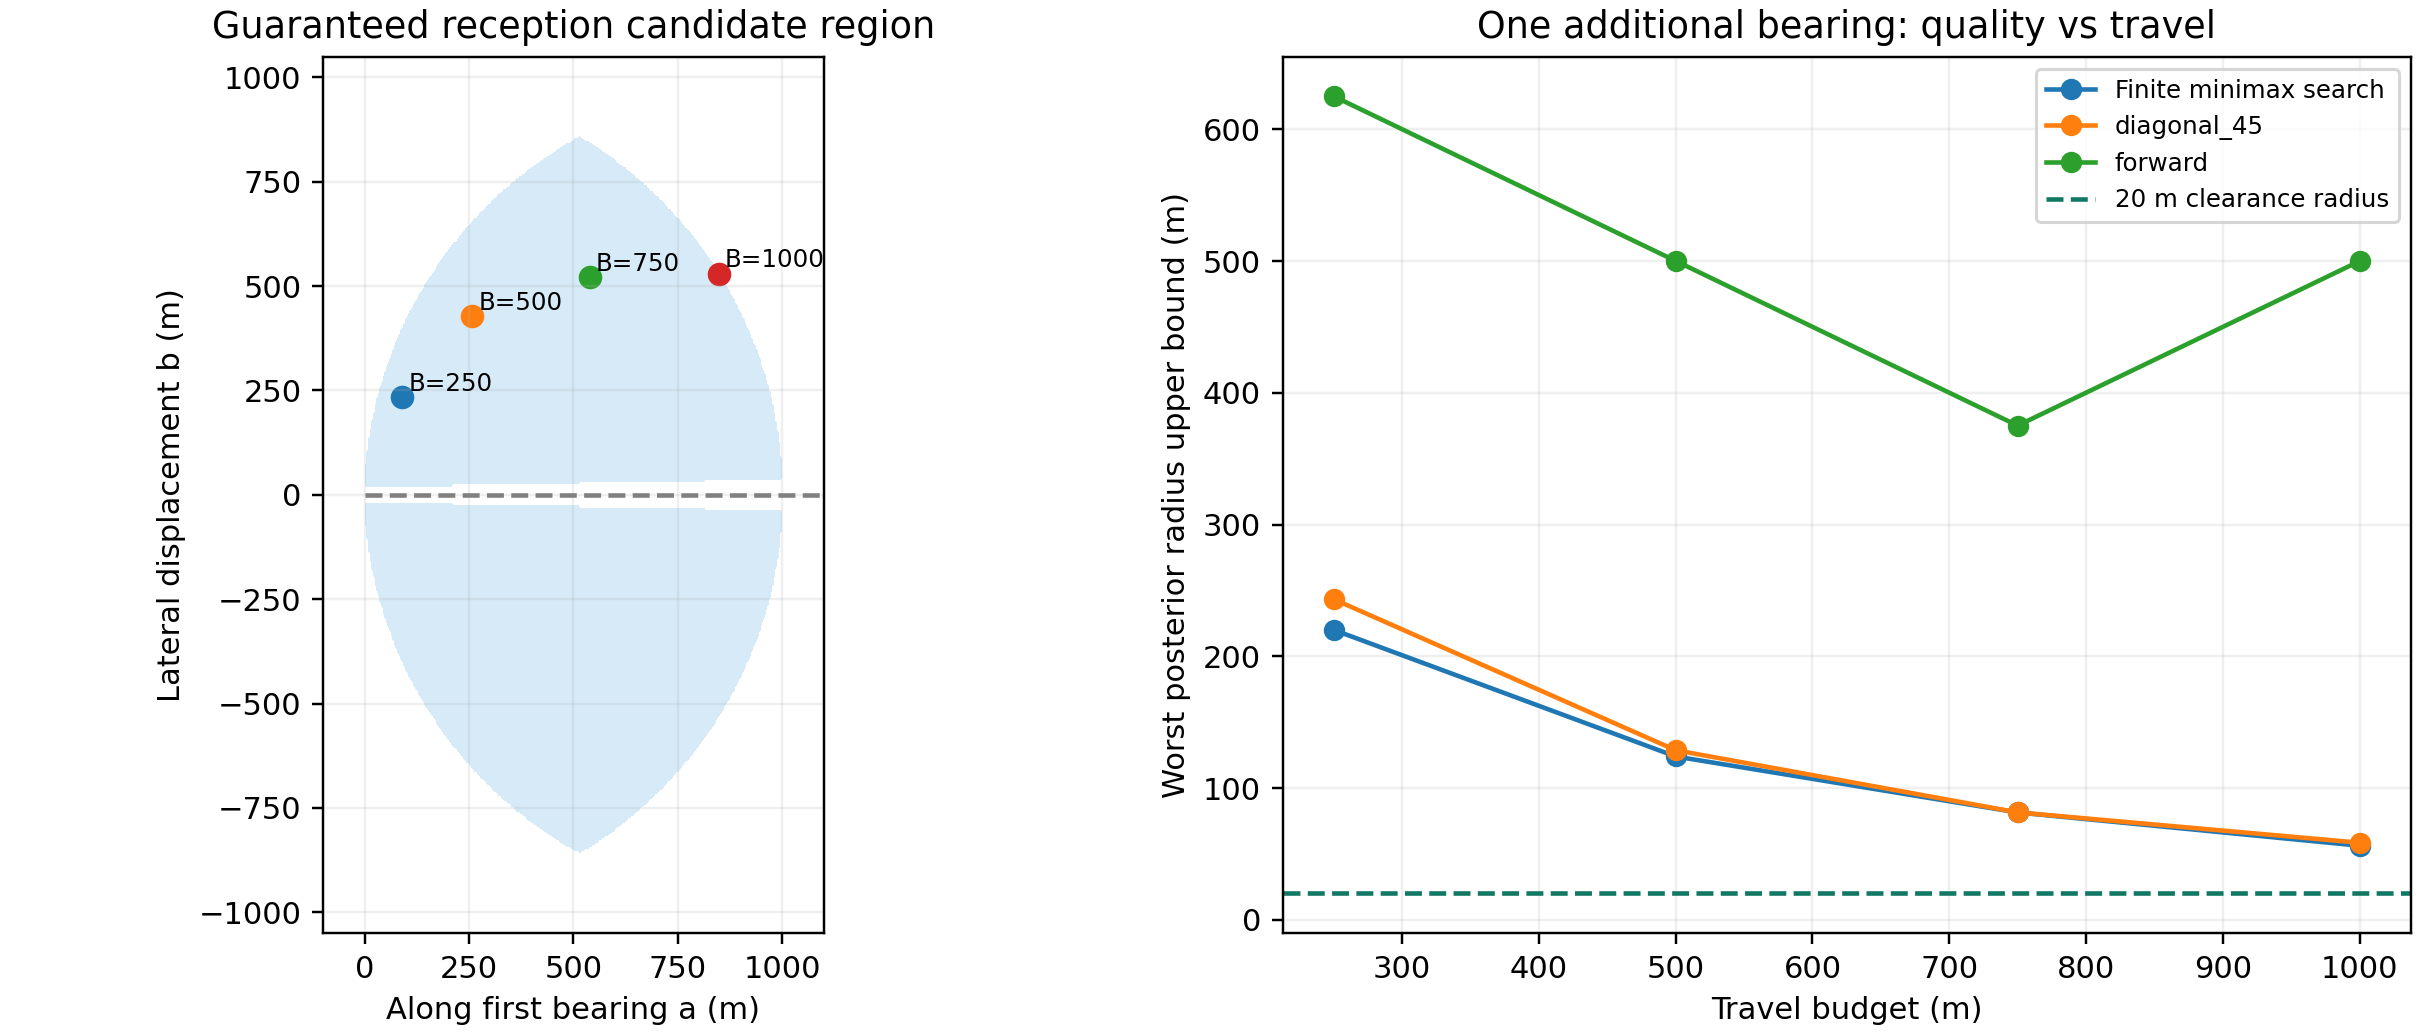
\includegraphics[width=0.94\textwidth]{q2-candidate-tradeoff.png}
  \caption{问题二的候选区域与精度—预算权衡。左：保证接收的三圆盘交集候选区域与四个预算下的推荐点；右：最坏后验包围圆半径 $U$ 随移动预算 $B$ 的变化，并与 $45^\circ$ 基线比较}
  \label{fig:q2-candidate}
\end{figure}

表 \ref{tab:q2-results} 展示的是"较多移动换取较低最坏不确定性"，并不意味着总任务越走越远越好。各预算下 $45^\circ$ 基线的上界依次约为 243.307、128.678、81.479、58.454 米；在 750 米预算下改进极小，因此不能夸大复杂优化相对简单几何规则的优势。

沿首次示向度前进的基线在未知距离下可能共线，残余半径明显较大；它仍可能对很近目标的抵近清除有价值，但本文只比较第二次测向的定位效果。纯横移基线没有接收保证，其报告值仅以"已获得第二个方向"为条件，不能与保证接收策略当作完整性能比较。

1100 条合成方向场景覆盖 11 种真实距离、5 种首次误差对应方向和 5 种第二次误差，每预算 275 条。所有推荐点均未失去信号，真实目标被后验包围圆包含，场景半径不超过连续分箱外包上界。需要说明：样本均值或可清除场景比例不代表官方环境中的期望性能。

图 \ref{fig:q2-range-stress} 给出真实距离变化下的场景压力检查。

\begin{figure}[H]
  \centering
  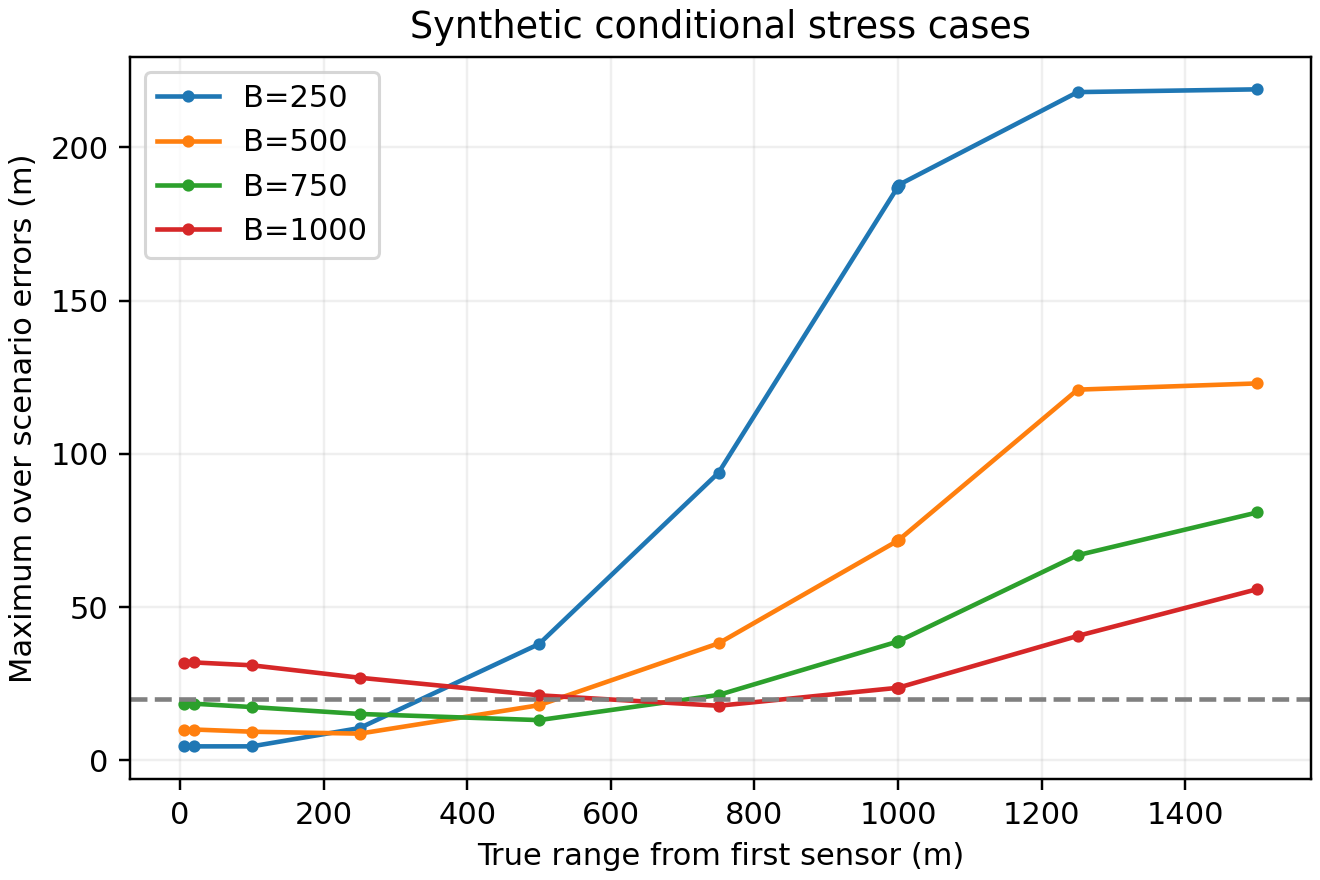
\includegraphics[width=0.86\textwidth]{q2-range-stress.png}
  \caption{问题二在真实距离变化下的压力检查。合成场景下后验半径随真实距离的变化及其与连续分箱外包上界的关系，该分布为本地设定，非官方概率分布}
  \label{fig:q2-range-stress}
\end{figure}

在最远距离条件下存在半径超过 20 米的实际合成后验，这不仅是上界松弛大于 20 米，而是确实存在无法由单个 20 米清除圆覆盖的后验区域。因此，这组具体策略不能普遍保证"只增加一次观测就可以清除"。但该事实不构成"所有可能的第二点策略都不可能做到"的全局不可能性证明。

\subsection{向后续问题提供的部件与改进方向}

可复用的部件包括：首次可行域、通用全向接收安全区域、按给定预算筛选第二点、观测后更新多边形外包、输出包围圆与清除充分条件。第三问可根据当前位置与其他目标选择 $B$，并在一个点复用多个频道的观测收益；本文未实现这些调度，也未将该一步精度目标冒充为总时间最优策略。第四问可复用角域更新、最小包围圆与清除判据，但\textbf{不能}复用式 \eqref{eq:K} 的全向接收保证——定向源的未知朝向引入额外的可见性条件，需另行建立。

值得保留的改进方向包括：利用圆域裁剪扩大 $K$；允许近距分支与直接清除，减少保守的横向限制；以"抵近与观测的总成本"替代单步精度；为连续空间搜索给出最优性差距；用更精细或自适应的读数箱降低保守度。这些方向本文尚未完成。

\section{问题三的模型建立与求解}

\subsection{任务条件与时间账本}

问题三的全部干扰源均为全向源，位置静止，频道唯一，接收半径未知但取值于 $[1000,1500]$ 米，总数 $N$ 未知且 $10\le N\le16$。机器狗自原点出发，初始检测频道为 1，移动速度 5 米/秒，清除操作不改变检测频道，也不要求返回原点。

在确保全部干扰源被清除的前提下，本文以虚拟总时间 $T$ 为优化目标。由式 \eqref{eq:time-ledger}，整场耗时可分解为移动、检测、换频与清除四项之和。该分解的意义在于把"少走路、少检测、少切频道、少失败尝试"放在同一时间尺度上，使局部决策不会因只优化其中一项而损害整体。需要说明的是，机器狗自身的计算时间不计入虚拟时间，但受题目给出的程序运行时间上限约束。

由于不同场景的目标数 $N$ 不同，跨场景对照一律采用\textbf{同一场景配对}；主指标为场景等权的均值 $K^{-1}\sum_j T_j/N_j$。本文另存合并比值 $\sum_jT_j/\sum_jN_j$ 用于核对，但不与场景等权均值混用。评测时不删除最后一次成功清除之后的必要搜索时间——在程序尚不知道 $N$ 的情况下，这段收尾是完成"确认无遗漏"所必需的。

\subsection{单源定位区域与保证清除}

对每个频道维护其全部正向测量历史，并求取凸外包多边形 $P$。先验取半径 1800 米圆域的外接正 180 边形；每次正向测量与半宽 $\varepsilon$ 的正向角域、以及以测站为中心半径 1500 米圆盘的外接多边形相交；近距（过强信号）记录与半径 5 米圆盘的外接多边形相交。角域半平面与最小包围圆的代码逐字复用问题一的实现并记录哈希。

角域半宽取 $\varepsilon=1.0051^\circ$，包含 $\pm1^\circ$ 的物理误差、读数保留两位小数带来的 0.005$^\circ$ 舍入以及 0.0001$^\circ$ 的数值余量。由假设五，同一位置的误差固定，不能通过在同一点重复测量来缩小误差。本文忽略近距记录对应的半径 5 米内部排除区，也忽略无信号记录产生的非凸排除区，这属于保守放宽，而不是把"无信号"当作"无目标"。

设 $P$ 的顶点为 $v_j$，最小包围圆为 $(c,\varrho)$。仅当 $\varrho\le19.5$ 米时才尝试有证书的清除；具体清除点 $q$ 满足
\begin{equation}
  \max_j\lVert q-v_j\rVert\le19.5 .
  \label{eq:q3-clear}
\end{equation}
对凸多边形，范数的最大值可在顶点取得，因此真实源到 $q$ 的距离不超过该上界，即不大于 19.5 米，留出 0.5 米的数值与工程余量。与问题一一致，$D(P)\le40$ 不能替代这一条件。

为节省路程，本文在"圆心 $c$ 指向机器狗当前位置 $p$"的线段上，用 45 次二分求最靠近 $p$ 的安全点；若 $p$ 已满足约束则原地清除。这是该线段上的最优点，不声称是全部安全清除点集到 $p$ 的全局投影。每次清除前保存顶点、点位与最坏距离证书；若接口返回失败，则保留冲突并退出，不得悄悄忽略。

\subsection{负观测的信息与接收半径约束}

无信号记录在第三问中携带两类信息。

\textbf{第一类：圆盘排除。} 若在位置 $n$ 未接收到某频道信号，则该源到 $n$ 的距离超过其接收半径，而接收半径不小于 1000 米，故可排除以 $n$ 为中心、半径 1000 米的圆盘。该操作通常产生非凸集；实现中使用
\begin{equation}
  \operatorname{conv}\Bigl(P\setminus\bigcup_{n\in S^-}\overline{B}(n,999.8)\Bigr)
  \label{eq:disk-exclusion}
\end{equation}
作为安全的凸外包，不把"圆外"误写成某个方向上的半平面。候选顶点由保留的多边形顶点、边与圆的交点、圆与圆的交点构成，过滤掉落在其他排除圆内或 $P$ 外的点后再求凸包。使用 999.8 米而非 1000 米提供数值余量。由于圆盘外侧边界对可行集而言是向内凹的，线性函数的最大值无需取其弧内部点。

\textbf{第二类：正负观测对生成的半平面。} 设 $s$ 为任一次有信号观测位置。由于同一个源的接收半径 $R$ 固定，有
\begin{equation}
  \lVert g-s\rVert\le R<\lVert g-n\rVert
  \;\Longrightarrow\;
  2(n-s)^{T}g<\lVert n\rVert^2-\lVert s\rVert^2 .
  \label{eq:pos-neg-halfplane}
\end{equation}
将每一对正、负观测生成的半平面加入 $P$，并使用向外 $10^{-6}$ 米的线性边界余量。该结论不要求接收半径恰为 1000 米，也不适用于接收半径随时间变化的模型。

\subsection{连续场地的停止证据}
\label{sec:coverage}

这是问题三中最关键、也最容易出错的部分。题目说明源总数在 10 至 16 之间但具体个数未知，因此\textbf{清除了 10 个或 14 个都不能结束}。本文只允许两种终止依据。

\textbf{依据一：}已清除 16 个源，达到题目给出的总数上界。

\textbf{依据二：}全部已发现源均已清除，并且每一个未发现频道都有全场覆盖证书。

覆盖证书的构造如下。将 $[-1800,1800]^2$ 等分为 $128\times128$ 个边长为 28.125 米的方格，保留所有与目标圆域相交的方格（含部分落在圆外的边界格）。对某个频道的一次无信号记录，只有当该方格\textbf{四个角点}到该无信号位置的距离都不超过 999.99 米时，才把整个方格标记为排除；由圆盘的凸性，这保证整格中的每一点都确实被排除。若某频道的全部保留方格均被其无信号记录覆盖，则该频道不可能存在源。

这一判据是\textbf{整格距离证书}，而不是仅检查网格中心的采样，两者有本质区别：后者在方格尺度较大时会漏掉真实的可能位置。

作为冗余核查，7 个外围测站的覆盖还可以直接验证：任一点与某个外围站的极角差不超过 $30^\circ$，比较其到原点及该外围站的距离，沿半径分段后最大最近站距离出现在半径 1800 米、角差 $30^\circ$ 的边界点处，约为 924.9 米，小于 1000 米。代码进一步对所有保留方格的完整覆盖进行独立检查。

此外还需注意两点。其一，发现 16 个不同频道后可以停止继续搜索未知频道，但仍必须清除这 16 个已发现源。其二，算法中"计划在某点扫描"只影响下一步的路线评分，\textbf{不写入实际排除记录}——未来覆盖不能当作已完成覆盖。

\subsection{发现—定位—清除闭环与联合路线}

\textbf{初始扫描。} 先在原点扫描所有尚未被排除的频道并缓存全部测量。同一位置的 20 个频道分别计时。

\textbf{任务点集合。} 把已知目标的安全清除点（或区域中心）作为必访点，把足以覆盖剩余场地的扫描点作为附加点。用固定起点、自由终点的最近邻路径初始化，再做 2-opt 改善顺序；每次实际观测后重新规划，只执行当前路线的第一项。因此这是一个滚动时域启发式，而不是全局最优动态规划。

\textbf{定位补测。} 初始设置一段 250 米的短基线用于同时改善多个已知目标的交会角。对已知频道的补测要求：距旧测点至少 150 米，区域尚不满足清除条件，且预计距离不超过 1200 米。对已有两次以上测量的目标，用中心方位及 $\pm1^\circ$ 三种假想读数预览区域收缩程度。需要强调，这个预览是补测价值的启发式估计，三种读数不是连续误差范围的最坏情况证书；真实清除仍使用完整的有界区域检查。

\textbf{扫描点的连续调整。} 从"目标中心加六个外圈站"构成的可行覆盖出发，逐一删除冗余扫描点。删除评分折算为移动距离：约 $30U$ 米（$U$ 为未发现频道数，每次检测近似 6 秒，速度 5 米/秒）的未知频道检测成本，加上可能缩短的局部路线。固定其余扫描站，对第 $i$ 站独占负责的剩余方格，取其全部角点的凸包顶点集 $V_i$，令前后路线点为 $a$、$b$，求解二维凸子问题
\begin{equation}
  \min_q\ \lVert q-a\rVert+\lVert q-b\rVert
  \qquad\text{s.t.}\quad \lVert q-v\rVert\le999.99\quad(\forall v\in V_i).
  \label{eq:scan-relocate}
\end{equation}
末站省略到 $b$ 的距离。将坐标缩放至千米后用 SLSQP 数值求解；只接受所有原始距离约束通过且局部目标不增加的结果，随后重新检查整体网格覆盖。不以求解器的成功标记代替可行性检查。删除、移动与路径重排组成交替改进；整体组合问题不是凸问题，本文不宣称全局最优。

\textbf{递推式的覆盖思路。} 上述覆盖构造借鉴了"首步可行 $\to$ 相邻步保持覆盖 $\to$ 末步覆盖边界 $\to$ 停止"的递推论证顺序，使任务完成有明确的判据，而不是"运行到次数上限"。但必须强调：连续测线在旧题中天然覆盖带内全部点，而本题中\textbf{走过一段路不等于在这段路上测过全部频道}；接收半径未知时，保证性论证只能使用已知下界 1000 米，不能使用 1500 米或样本平均半径。

\subsection{光学动作的时间价值}

在定位区域已经足够小时，直接进行一次光学试探可能比继续测向更省时间。本文仅在 $19.5<\varrho\le100$ 米时比较试清动作。候选位置包括当前位置、包围圆中心、朝当前机器狗偏移的点以及长轴两侧的点，每源最多试探两次；位置信息表示点来自当前的非凸可行集 $F$ 而非模拟器真值。

\textbf{非凸失败信息的保留。} 已知源在 $q$ 点清除失败意味着 $\lVert g-q\rVert>20$，这是一条有效信息。本文在数值实现中移除"半径 19.999 米圆盘的内接 64 边形"，所得删除区域严格包含在真实可排除范围内，因而留下的仍是外包集合。实现保持两种表示：非凸集合 $F$ 保存全部光学失败排除，$\operatorname{conv}(F)$ 的顶点用于原有测向、接收与最小包围圆计算；后续正向测向区域与 $F$ 相交，不以凸包覆盖 $F$ 的存储。保留所有连通分量与孔洞。

\textbf{动作评价。} 对动作 $a$ 与代表情景 $h$，评价量取
\begin{equation}
  C(a,h)=\frac{\text{移动距离}}{5}+\text{本动作检测或清除费用}+\text{后续常规定位完成费用},
  \label{eq:action-value}
\end{equation}
其中试清成功计 5 秒、失败计 3 秒并使用更新后的区域预测后续费用。无线电预测每次按 6 秒保守计入切换，而实际模拟按真实频道计费。预测使用至多 5 步原几何定位；评价取 $0.8$ 倍情景均值加 $0.2$ 倍情景最大值，且至少比无线电方案少 1 秒才尝试试探。需要说明：均值权重与代表情景都是规划约定，不是概率模型，也不是连续最坏情形的证明；预测并未完整建模试清后对整场路径的影响，因此最终必须经实际全场验证。这一"先看本轮动作如何影响未来，再向后试算若干步"的组织方式，参考了往年优秀论文中有限步状态更新与"当前成本加后续成本"的论证结构，但本题的物理条件与计费规则均按今年附件重新建立，原论文中的免费多目标观测、概率噪声与全局真值假设均未沿用。

\subsection{求解结果}

\subsubsection{同场配对审计}

本文使用固定随机种子的合成场景集进行同场配对比较，所有结果均计入整场末尾排除与失败清除费用。

\begin{table}[H]
  \centering
  \caption{问题三的同场配对审计结果（场景等权 $T/N$，单位：秒/点）}
  \label{tab:q3-results}
  \begingroup
  \renewcommand{\arraystretch}{1.4}
  \begin{tabularx}{\textwidth}{L{0.34\textwidth}C{0.11\textwidth}C{0.14\textwidth}C{0.14\textwidth}C{0.13\textwidth}}
    \toprule[1.2pt]
    {\heifont\bfseries 测试组} & {\heifont\bfseries 场数} & {\heifont\bfseries 对照版} & {\heifont\bfseries 本模型} & {\heifont\bfseries 平均改善} \\
    \midrule[0.5pt]
    200 场同场审计（联合规划 vs 基线） & 200 & 317.38 & 237.19 & 25.27\% \\
    100 场三版本对照（v3 / v4 / v5） & 100 & 238.11 & 234.23 & 1.63\% \\
    60 场冻结配对（v5 $\to$ v6 光学评价） & 60 & 234.03 & 232.60 & 0.61\% \\
    \bottomrule[1.2pt]
  \end{tabularx}
  \endgroup
\end{table}

在 200 场同场配对审计中（种子 5100--5299），基线、区域耦合、连续覆盖与组合方案的场景等权均值依次为 317.38、238.71、238.40、237.19 秒/点；四套方案全部实现 200/200 完整清除、零失败清除，配对均值的近似 95\% 区间为 $[232.52,241.85]$ 秒/点。需要说明：该区间只表示给定本地生成规则下的场景抽样不确定性，\textbf{不是}官方泛化区间。

在 100 场三版本同场对照中，v3、v4、v5 分别为 238.1110、234.8970、234.2317 秒/点，全部完整清除、零失败清除。v4 与 v5 的配对均值差为 0.6652 秒/点，近似 95\% 区间为 $[-1.8046,3.1351]$，包含 0；因此\textbf{不能认定 v5 相对 v4 具有稳定优势}。这一轮实验中平均每场少走 322.15 米但多检测 8.93 次，测量费用抵消了大部分移动收益，这为"补测价值估计"这一后续方向提供了证据。

在 60 场冻结留出配对中（种子 17000--17059），加入光学动作评价的 v6 相对 v5 由 234.03 降至 232.60 秒/点，平均节省 1.4283 秒/点（0.61\%），配对近似 95\% 区间为 $[1.0976,1.7591]$，54 场改善、6 场退化，最差场景（种子 17020）增加 1.7588 秒/点。本轮平均路程由 10833.10 米降至 10816.56 米，检测次数由 123.28 降至 118.73 次，新版平均发生 3.33 次失败光学尝试，其时间代价均已计入。

\begin{figure}[H]
  \centering
  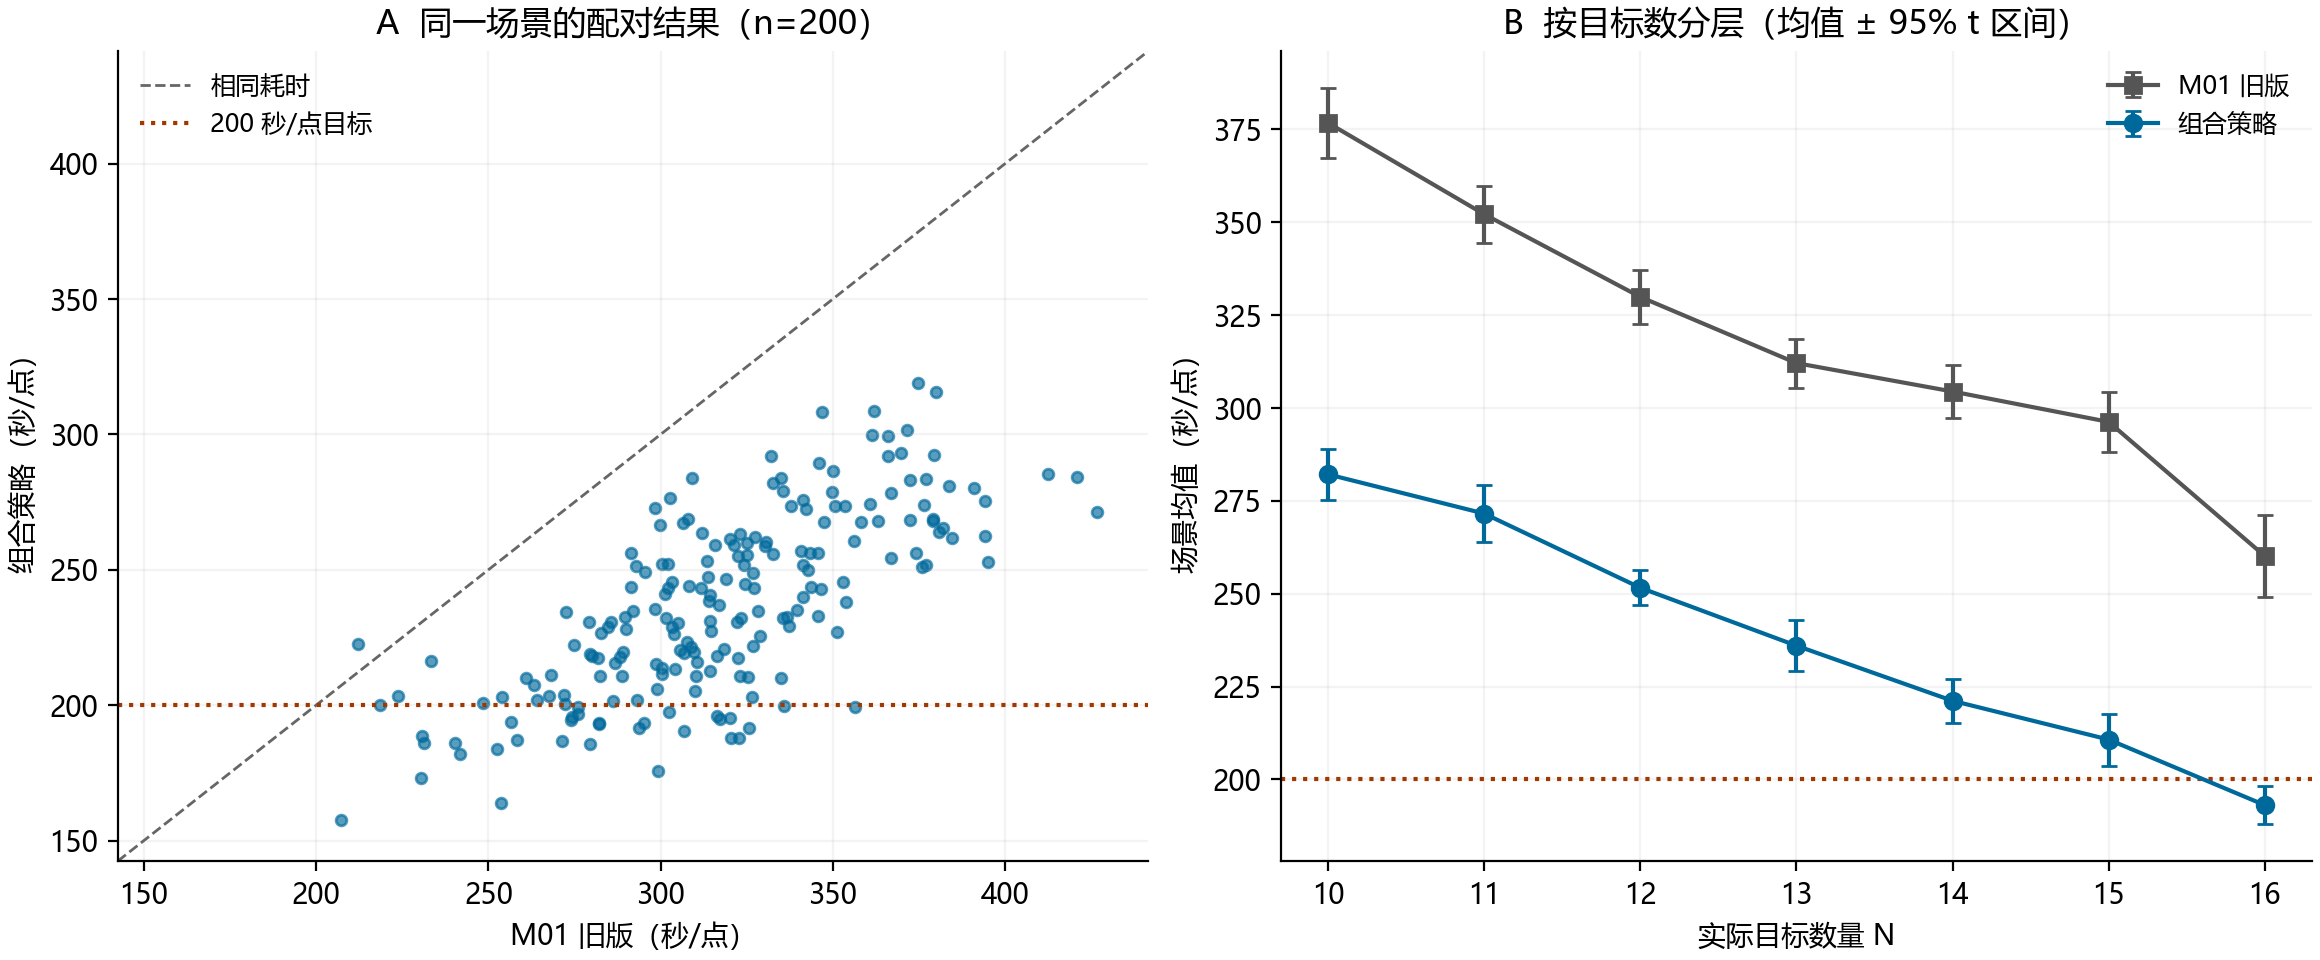
\includegraphics[width=0.94\textwidth]{q3-joint-paired.png}
  \caption{问题三的逐场配对比较。200 场同场审计中各方案相对基线的每场时间变化与累计分布，含末尾排除与失败清除费用}
  \label{fig:q3-joint}
\end{figure}

\subsubsection{真实官方演练}

在本地合成实验之外，本策略完成了一次真实的官方演练，案例编码 JCEK-BMVS-WD8Z-WF6J。官方结果文件确认场内共有 14 个全向干扰源；动作响应确认成功清除 14 个、零失败，正常主动退出。总虚拟时间 3854.083567 秒，平均每源 275.29 秒，累计移动 16020.418 米。全部数据来自保存的官方接口响应，并已按原始动作独立重算；未解密官方日志，也未连接或重跑模拟器。

\begin{table}[H]
  \centering
  \caption{问题三官方演练的时间分解（案例 JCEK-BMVS-WD8Z-WF6J，14 个全向源）}
  \label{tab:q3-official}
  \begingroup
  \renewcommand{\arraystretch}{1.4}
  \begin{tabularx}{\textwidth}{L{0.34\textwidth}C{0.18\textwidth}C{0.16\textwidth}Y}
    \toprule[1.2pt]
    {\heifont\bfseries 计费项} & {\heifont\bfseries 虚拟时间/秒} & {\heifont\bfseries 占比} & {\heifont\bfseries 次数} \\
    \midrule[0.5pt]
    移动            & 3204.084 & 83.13\% & 累计 16020.42 米 \\
    检测            & 495.000  & 12.84\% & 99 次 \\
    检测频道切换    & 85.000   & 2.21\%  & 85 次 \\
    成功清除        & 70.000   & 1.82\%  & 14 次 \\
    清除失败        & 0.000    & 0.00\%  & 0 次 \\
    \midrule[0.5pt]
    合计            & 3854.084 & 100.00\% & 115 个唯一动作 \\
    \bottomrule[1.2pt]
  \end{tabularx}
  \endgroup
\end{table}

本局共发出 115 个唯一动作（进入 1、检测 99、清除 14、退出 1），115 个请求与 115 个响应全部一次接受，无重试、拒绝或未确认动作；逐动作时间守恒的最大偏差为 $4.87\times10^{-7}$ 秒，符合响应的小数舍入。39 次正向观测中，14 次为首次发现，其余 25 次为定位补测，即每个源平均新增 1.79 次定位检测。按动作用途划分，扫描点检测 74 次、专门定位检测 25 次。最后一次清除发生在 3292.188 秒，之后用去 561.896 秒（占全程 14.58\%）完成余下两个测站、12 次无信号检测。

这一收尾段不是可以直接删除的浪费：程序当时并不知道总数为 14，仍需排除其他频道；第 4 个测站虽然没有发现新源，但其无信号记录参与了完整覆盖证书。这正说明了第 \ref{sec:coverage} 节终止依据的必要性。

\begin{figure}[H]
  \centering
  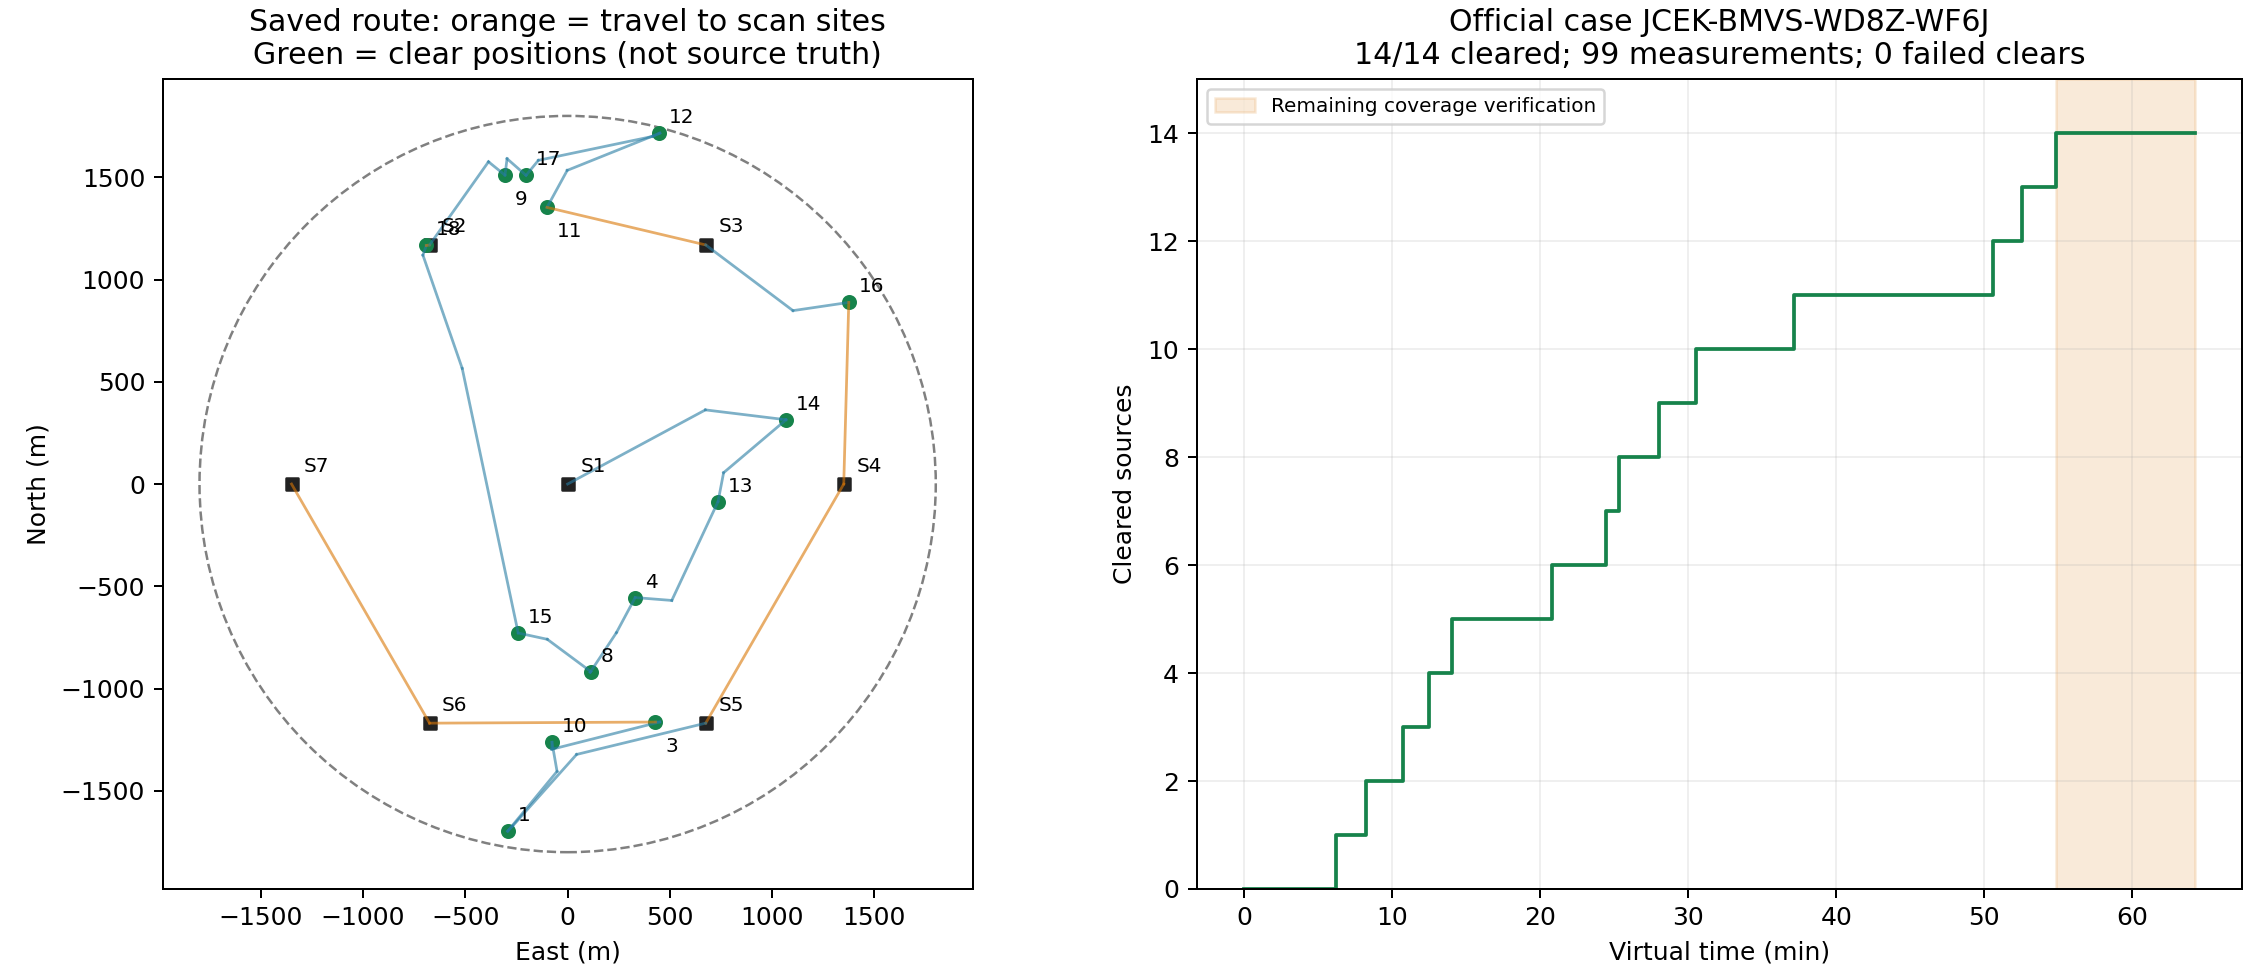
\includegraphics[width=0.88\textwidth]{q3-official-route.png}
  \caption{问题三官方演练的实际轨迹与清除进度。绿色标记为清除动作发生位置，其中部分为原地近距清除；图中标记是清除点而非干扰源真实坐标}
  \label{fig:q3-official-route}
\end{figure}

图 \ref{fig:q3-official-route} 给出该局的轨迹与逐源清除进度。需要特别指出，图中的清除标记是机器狗执行清除时的位置（距真实源不超过 20 米），\textbf{不能当作干扰源的真实坐标}。

\subsubsection{与前次演练的比较及可比性说明}

本策略另与两次更早的演练记录作了对比，结果见表 \ref{tab:q3-history}。

\begin{table}[H]
  \centering
  \caption{问题三三次官方演练记录对比}
  \label{tab:q3-history}
  \begingroup
  \renewcommand{\arraystretch}{1.4}
  \begin{tabularx}{\textwidth}{L{0.26\textwidth}C{0.10\textwidth}C{0.13\textwidth}C{0.12\textwidth}C{0.10\textwidth}C{0.10\textwidth}}
    \toprule[1.2pt]
    {\heifont\bfseries 演练} & {\heifont\bfseries 已清除} & {\heifont\bfseries 总虚拟时间/秒} & {\heifont\bfseries 每源平均/秒} & {\heifont\bfseries 路程/km} & {\heifont\bfseries 清除失败} \\
    \midrule[0.5pt]
    20260910-200250 & 14 & 6446.68 & 460.48 & 27.248 & 11 \\
    20260910-222119 & 16 & 6684.96 & 417.81 & 27.595 & 15 \\
    20260911-002124（本策略） & 14 & 3854.08 & 275.29 & 16.020 & 0 \\
    \bottomrule[1.2pt]
  \end{tabularx}
  \endgroup
\end{table}

相对第一局 14 源旧演练，本局总时间低 40.22\%、路程少 41.21\%；相对第二局 16 源旧演练，每源平均时间低 34.11\%。\textbf{但这三局的案例并不相同}，目标数相同也不代表场景相同，因此这些差值不能作为策略因果提速的证据，也不能替代同案例配对比较。本文将其列为实际运行记录，仅用于说明策略在真实接口上可完整运行。

\subsection{有效性检验与未达标说明}

\textbf{几何与动作的独立核验。} 对演练日志，本文重建了 39 次正向观测的完整约束，对每个区域做 16 方向线性规划支持函数检查共 624 项，最大差异 $1.23\times10^{-11}$ 米；14 次清除点全部通过顶点最坏距离复核。对未发现的频道 2、5、6、7、19、20，均有 7 个测站的真实无信号记录，从动作记录重新构造的整格覆盖最小半径余量为 60.621 米——这一结论不是仅相信摘要中的完成标志。

\textbf{压力与消融测试。} 第三问的边界布局、固定极端测角误差（恒定 $+1^\circ$ 与 $-1^\circ$）以及棋盘式误差场测试均实现完整清除，但极端误差组略慢、棋盘误差组几乎持平（-0.00\%）。20 场消融实验中，"不更新失败区域"为 238.0196 秒/点，"更新失败区域"为 237.9988 秒/点，差值仅 0.0208，区间 $[-0.3224,0.3640]$；因此\textbf{不能把整体提速归因于失败信息更新这一单项}——它在几何上是有效的，但效率贡献尚未被证实。

\textbf{200 秒/点目标未达成。} 需要如实说明：本轮全部讨论中出现的"200 秒/点"是团队设定的内部研究目标，并非题目要求。当前方案未达到该目标。进一步地，本文构造的圆周 10 源场景给出移动下界 233.64 秒/点，这否定了"在全部合法场景上获得 200 秒硬保证"的可能性；但这\textbf{不}否定特定分布下均值可能降至 200 秒，本文也没有证明该分布均值不可达。

此外，16 个源子组的平均 193.09 秒/点不能替代全体场景的 237.19 秒/点。不能选择容易场景、忽略失败或删去收尾段后宣称达成目标。

\textbf{剩余的主要研究方向}是跨源定位任务、停靠位置与未来路径的联合选择。本轮的局部完成费用预测不能称为完整的多步全局规划，独立审计也显示当前局部成本的改善并没有稳定减少整场移动距离。

\subsection{正式测试结果}

按题目要求，需在充分演练后进行三次正式测试，并按表 1 的格式给出结果。

\begin{table}[H]
  \centering
  \caption{问题三正式测试结果}
  \label{tab:q3-formal}
  \begingroup
  \renewcommand{\arraystretch}{1.45}
  \begin{tabularx}{\textwidth}{L{0.22\textwidth}C{0.18\textwidth}C{0.20\textwidth}C{0.20\textwidth}}
    \toprule[1.2pt]
    {\heifont\bfseries 测试案例编码} & {\heifont\bfseries 清除干扰源个数} & {\heifont\bfseries 平均定位清除时间} & {\heifont\bfseries 程序运行时间} \\
    \midrule[0.5pt]
    测试1 \hspace{2em} & \hspace{2em} & \hspace{2em} & \hspace{2em} \\
    测试2 \hspace{2em} & \hspace{2em} & \hspace{2em} & \hspace{2em} \\
    测试3 \hspace{2em} & \hspace{2em} & \hspace{2em} & \hspace{2em} \\
    \bottomrule[1.2pt]
  \end{tabularx}
  \endgroup
\end{table}

\textbf{截至本文写作时，三次正式测试尚未进行，表 \ref{tab:q3-formal} 的内容留空。} 本文已有的全部第三问数值均来自本地合成场景与一次官方演练，不构成正式测试成绩。相应地，正式测试对应的三份模拟器日志文件也将在测试完成后导出并放入支撑材料。

\section{问题四的模型建立与求解}

\subsection{第四问改变了哪些条件}

问题四在问题三的基础上引入定向干扰源：源总数仍为 10 至 16 个且未知，但现在既有全向源又有定向源，定向源的个数与朝向也未知。由附录一，定向源的有效覆盖角度为发射方向两侧各 $90^\circ$（含边界），范围之外没有信号辐射；而光学精确定位与清除只受 20 米距离约束，与源的朝向无关。

以 $g$ 表示源位置、$R$ 表示接收半径、$n=(\cos\varphi,\sin\varphi)$ 表示定向源的发射方向单位向量、$\tau\in\{\text{全向},\text{定向}\}$ 表示类型，则位置 $s$ 能接收到某个未清除源，当且仅当
\begin{equation}
  \lVert s-g\rVert\le R
  \quad\text{且}\quad
  \bigl[\tau=\text{全向}\ \text{或}\ n^{T}(s-g)\ge0\bigr].
  \label{eq:directional-reception}
\end{equation}
需特别注意：示向度是 $s$ 指向 $g$ 的角度，\textbf{不是}发射方向 $\varphi$。因此由示向度不能推断源的类型或朝向；由无信号也不能认定附近没有源。

据此逐项检查第三问的机制，得到表 \ref{tab:q4-inherit} 的继承清单。这张清单是第四问建模的起点：真正需要重新建立的只有"无信号的含义"与"覆盖终止证书"两项，其余几何与清除模块可以原样继承。

\begin{table}[H]
  \centering
  \caption{第三问机制在第四问中的继承情况}
  \label{tab:q4-inherit}
  \begingroup
  \renewcommand{\arraystretch}{1.4}
  \begin{tabularx}{\textwidth}{L{0.36\textwidth}Y}
    \toprule[1.2pt]
    {\heifont\bfseries 第三问机制} & {\heifont\bfseries 第四问的处理} \\
    \midrule[0.5pt]
    有界示向度半平面、多边形外包、最小包围圆 & 收到信号时继续成立，原样继承 \\
    最近保证清除点计算 & 光学不受朝向限制，直接继承 \\
    全向接收候选区域（问题二） & 只解决距离条件，\textbf{不能}承诺定向接收 \\
    无信号排除 1000 米圆盘 & \textbf{禁用}：定向源可能就在旁边但背向 \\
    全向覆盖终止证书 & 更换为对任意朝向成立的三角网证书 \\
    联合路线、每次补测计费、完整尾部统计 & 继承其原则 \\
    \bottomrule[1.2pt]
  \end{tabularx}
  \endgroup
\end{table}

一个说明"外侧扫描为何必要"的极端例子是：源位于 $g=(1800,0)$、朝向 $n=(1,0)$。此时严格位于场地内部的点全部处于其发射半平面的后方，仅在场内扫描没有任何发现保证。因此允许机器狗走出半径 1800 米的源分布区域是覆盖逻辑的内在需要，而不是数值越界；题目附件亦明确允许场外位置。

\subsection{状态表示与更新}

机器狗的状态为当前位置 $p$、当前检测频道 $c$、已发现频道集合 $D$ 与已清除频道集合 $C$。未知频道指尚未被发现、也尚未被证明不存在的频道。历史动作按频道保存其位置与真实响应；仅经过某点不计作检测。

评价仍以虚拟总时间为目标，形式与式 \eqref{eq:time-ledger} 相同：
\begin{equation}
  T=\frac15\sum_k\lVert p_k-p_{k-1}\rVert+5M+S+5C_s+3C_f ,
  \label{eq:q4-time}
\end{equation}
其中 $M$ 为检测次数，$S$ 为检测频道切换次数，$C_s$、$C_f$ 分别为成功与失败的光学操作次数。清除操作不改变检测频道，不要求返回原点。评价同时报告清除完整率与 $T/N_{\text{clear}}$；本地全清场景以真实 $N$ 计算 $T/N$ 并对场景等权平均，未清完场景的低时间不得当作有效速度。

完整的物理可行状态可写作 $(g,R,n,\tau)$ 的集合 $\Omega$。正向观测交入接收条件与测角约束；负向观测交入
\begin{equation}
  \lVert s-g\rVert>R
  \quad\text{或}\quad
  \bigl[\tau=\text{定向},\ n^{T}(s-g)<0\bigr].
  \label{eq:neg-obs}
\end{equation}
该析取导致联合状态非凸。本文不声称精确求解 $\Omega$，而是分开保存以下两类表示。

\textbf{可靠位置外包 $P$。} 初始为 1800 米圆域的 180 边外接多边形；正向观测交入半宽 $\varepsilon=1.0051^\circ$ 的前向角域与半径 1500.000001 米圆盘的外接多边形；近距记录交入半径 5.000001 米圆盘的外包。保留 0.005$^\circ$ 舍入余量与微小数值余量。\textbf{无信号记录只记入历史，不对 $P$ 做任何圆盘删减。} 真实位置应始终包含在 $P$ 中。

\textbf{规划用有限假设 $H$。} 取 $P$ 内的顶点与内部插值位置，对每个位置采样至多 3 个接收半径与 72 个朝向，并保留全向假设。历史负观测按"超出距离或处于背面"进行筛选。相容样本中"可接收"的比例只用于动作评分，它不是经过校准的真实概率，也不穷尽连续可行状态。样本为空只表示当前离散表示不足，\textbf{不代表源不存在}；此时评分回退为 0.5 并继续保留 $P$。

近距离观测可直接检查安全清除；接收半径未知与类型未知都不影响光学操作。

\subsection{对任意朝向成立的发现证书}
\label{sec:q4-mesh}

用边长 $L=990$ 米的等边三角网覆盖场地，基向量为 $(990,0)$ 与 $(495,495\sqrt3)$。保留与半径 1800.01 米圆域相交的全部三角形，并保留其全部顶点。实现共生成 31 个点、42 个三角形，其中 18 个点位于圆域之外；0.01 米为边界数值余量，不扩大源先验。

\textbf{定理。} 任取三角形顶点 $s_1,s_2,s_3$ 及三角形内的源位置 $g$，存在非负系数 $\lambda_i$ 且 $\sum_i\lambda_i=1$ 使 $g=\sum_i\lambda_is_i$。对任意朝向 $n$，有
\begin{equation}
  \sum_{i=1}^{3}\lambda_i\,n^{T}(s_i-g)
  =n^{T}\Bigl(\sum_i\lambda_is_i-g\Bigr)=0 .
  \label{eq:convex-comb}
\end{equation}
因此三个内积不可能都严格小于 0，至少有一个顶点位于源的闭发射半平面内。又因三角形中任意两点距离不超过 $L=990$ 米，小于接收半径下界 1000 米，所以该顶点能够接收到该源的信号；全向源自然也满足。$\square$

\textbf{推论。} 若某频道在某个三角形的三个顶点都实际测得无信号，则该三角形内不存在此频道的源。当全部三角形都满足该条件时，整个场地被排除。

这里必须登记完全相同的网格坐标，不能用邻近但不同的检测点替代顶点，否则会破坏角度边界处的凸组合依据。

作为一个可人工核验的例子：取 $s_1=(0,0)$、$s_2=(990,0)$、$s_3=(495,\,857.3651497)$，源位于重心 $g=(495,\,285.7883832)$，三个顶点到 $g$ 的距离均约为 571.5768 米。当 $n=(0,-1)$ 时，前两个顶点的内积为 $285.7884>0$，第三个为 $-571.5768$，即至少有一个顶点可接收，且都在 1000 米以内。形式证明对任意位置与任意朝向成立，不依赖这个例子，也不依赖朝向的离散采样。

该网格给出的是保守充分条件，不是必要条件，也不是最优站点布局。

\subsection{凸包排除定理与 22 点布局}

三角网证书要求三个顶点都实际无信号。实践中可以放宽为更一般的条件。

\textbf{定理（凸包排除）。} 设 $Q$ 为一个凸子区域，$S_Q$ 为同一频道的实际无信号点集合，且 $S_Q$ 中每个点 $s$ 到 $Q$ 的每个顶点的距离都不超过 999.99 米。由欧氏距离的凸性，这保证每个 $s$ 到 $Q$ 内所有点的距离都不超过该范围。若 $Q\subseteq\operatorname{conv}(S_Q)$，则 $Q$ 中不存在任何朝向的该频道源。

\textbf{证明。} 反设 $Q$ 中存在一个定向源位于 $g$，则其全部无信号点必须满足 $n^{T}(s-g)<0$。但 $g\in Q\subseteq\operatorname{conv}(S_Q)$，故 $g$ 是这些 $s$ 的凸组合；取相同权重求和得 $n^{T}(g-g)=\sum_i\lambda_in^{T}(s_i-g)<0$，即 $0<0$，矛盾。全向源更直接由距离条件排除。半平面边界包含在可接收区域内，是推导的必要条件。$\square$

原先的 31 点三角网只是该定理在固定三角网下的一种特例。新算法允许子区域 $Q$ 的不同顶点由不同的三点组合证明，只要各组合的站点都满足"到整个 $Q$ 的距离条件"即可得到 $Q$ 属于所有这些站点凸包的结论。需注意：不能仅分别证明每个顶点可被排除，而忽略整个 $Q$ 的距离条件。

\textbf{布局构造。} 据此，本文选取：中心 1 点 $(0,0)$，半径 980 米的等角内圈 7 点，半径 1850 米的等角外圈 14 点，均从正 $x$ 方向起算，共 22 个站点，替代原先的 31 点网格。以原三角网覆盖作为分区起点，每个三角形与半径 1800 米圆的外切 360 边形相交（不能用内接多边形替代场地）；对无法直接获得凸包证据的三角形递归四分。22 点构造共得到 1334 个通过条件的凸子区域并覆盖整个连续场地；25 点备选方案得到 722 个子区域但选择集效率低于 22 点，保留为备选；19 点与 21 点的更少点候选未通过当前几何条件。

执行器预先计算三点组合对每个子区域顶点的证据，并用位集加速实际负观测组合的查询。只有\textbf{真正执行过}且返回无信号的站点才能用于结束证明；未来站点在路径规划时可暂按无信号计算预期覆盖，但不进入完成证书。发现 16 个频道后不再搜索未知频道，但仍必须清除全部已发现源。

本轮的主要收益假设是：减少站点数量，并把原先最外层 2619 米的站点移至 1850 米圈，从而同时减少移动距离与搜索检测次数。这一假设必须由同场路径与检测账目支持，不能仅凭站点数量的下降认定时间改善。

\subsection{发现—定位—清除闭环}

\begin{enumerate}[label=(\arabic*),leftmargin=2.2em]
  \item 在原点逐频道扫描；同一位置的 20 个频道仍分别计时。近距记录立即清除。
  \item 将仍需要扫描的网格站点与已发现未清除源的区域中心作为任务点，构造固定起点、自由终点的路线；最近邻初始化后最多做 30 轮 2-opt，只执行当前路线的第一项，观测后重新计算。
  \item 若任务为扫描，则检测尚未被排除、且从未在该顶点返回负观测的未知频道；默认不附加已知频道的测量。
  \item 若任务为定位，先求保证清除点，若存在则执行。否则在区域中心、长轴两侧、末次正向观测点向区域中心前进 45\% 与 75\% 的位置以及侧移点中选下一测点，排除与历史测点距离不足 8 米的位置。
  \item 连续 3 次无信号或 10 次局部观测仍未达到清除精度时，转入光学区域后备，不靠原地重测或强行删除区域来结束。
  \item 已发现 16 个不同频道后立即停止未知频道搜索，只完成已知源；清除 16 个后结束。若不足 16 个，则必须所有已知源均已清除，且每个其余频道都有全场排除证书，才能结束。
\end{enumerate}

路线中的区域中心是服务位置的近似，并未完整预测定位进入点与清除退出点，因此它不是全局在线最优路线。

\subsubsection{下一测点的时间评分}

对候选点 $q$，记 $H$ 中可接收比例估计为 $\hat p$，围绕预测中心方位的 $-1^\circ$、$0^\circ$、$+1^\circ$ 三个假想读数给出平均区域半径 $\hat r'$。它们只估计测量收益，\textbf{不是}所有可能读数下的严格最坏情况。再记位置中心为 $c$、末次正向观测位置为 $s^+$、当前包围半径为 $\varrho$，评分取
\begin{equation}
  J(q)=\frac{\lVert p-q\rVert}{5}+6
  +\hat p\Bigl(\frac{\lVert q-c\rVert}{5}+\frac{2\hat r'}{5}\Bigr)
  +(1-\hat p)\Bigl(\frac{\lVert q-s^+\rVert}{5}+\frac{2\varrho}{5}+20\Bigr).
  \label{eq:q4-score}
\end{equation}
选择分数最小的点。式中距离系数 $1/5$ 来自移动速度；固定项 6 秒近似一次检测与换频（同频道实际仅 5 秒，但该公共项不改变同频道候选之间的排序）；$2\varrho$ 用于近似剩余定位行程；20 秒为失联处理的工程惩罚，不是题目给定参数，也不是对真值的估计。侧移距离 $\max(30,\min(180,0.3\varrho))$ 同样是工程参数。所有真正执行的动作费用按接口重新记账。该评分把第三问"少走路却多测、抵消收益"的经验用于决策，但当前只实现了局部评分，其权重仍需通过后续消融与官方演练检验。

\subsection{清除与光学后备}

常规清除采用 $\mathcal{K}=\bigcap_{v\in\text{vertices}(P)}\overline{B}(v,19.5)$。若 $\mathcal{K}$ 非空，选择距机器狗最近的点 $q\in\mathcal{K}$；对凸多边形，距 $q$ 的最大值在顶点取得，故真实源到 $q$ 的距离不超过 $19.5<20$ 米。已认证清除若执行失败，则记录冲突并停止，不能继续宣称保证。

光学后备搜索把 $P$ 投影到其直径方向的坐标系，以边长 26 米的正方格覆盖，保留所有与 $P$ 相交的方格，在每个方格中心尝试一次清除。每格内任一点到格心的距离不超过 $13\sqrt2\approx18.3848$ 米，故当全部方格被覆盖时必有一次成功，且该结论与源的发射朝向无关。实际采用最近邻次序，成功即停；失败的尝试各支付 3 秒及相应移动费用。它是有限覆盖搜索，不是每一次尝试都保证成功，也不被伪装成零失败清除。

上述完整性逻辑在题面静态物理条件成立、观测误差界成立、动作能正常执行且未被现实或虚拟预算截断时有效。数值几何采用浮点与外包余量，并非形式化区间算术证明；预算中止或异常必须作为未完成状态保存。

\subsection{求解结果}

在 40 场冻结留出配对中（种子 26000--26039），原 31 点网格策略与 22 点布局策略使用完全相同的场景。

\begin{table}[H]
  \centering
  \caption{问题四 40 场冻结配对结果（场景等权 $T/N$，单位：秒/点）}
  \label{tab:q4-main}
  \begingroup
  \renewcommand{\arraystretch}{1.4}
  \begin{tabularx}{\textwidth}{L{0.30\textwidth}C{0.14\textwidth}C{0.14\textwidth}C{0.14\textwidth}Y}
    \toprule[1.2pt]
    {\heifont\bfseries 策略} & {\heifont\bfseries 时间/秒} & {\heifont\bfseries 平均路程/米} & {\heifont\bfseries 平均检测次数} & {\heifont\bfseries 说明} \\
    \midrule[0.5pt]
    31 点网格（原版） & 696.78 & 36537.13 & 312.43 & 全部完整清除 \\
    22 点布局（本模型） & 515.63 & 26611.70 & 249.95 & 全部完整清除 \\
    \midrule[0.5pt]
    平均节省 & 181.15 & 9925.43 & 62.48 & 降低 26.00\% \\
    \bottomrule[1.2pt]
  \end{tabularx}
  \endgroup
\end{table}

40 场平均由 696.78 秒/点降至 515.63 秒/点，节省 181.15 秒/点，降低 26.00\%；配对节省的近似 95\% 区间为 $[151.78,210.53]$ 秒/点。40 场中 39 场改善、1 场退化。平均路程由 36537.13 米降至 26611.70 米，平均检测次数由 312.43 次降至 249.95 次。

\textbf{必须报告退化案例。} 最差场景（种子 26011）反而增加 145.79 秒/点；该场的源数 $N=16$，原策略较早发现了全部频道而提前停止搜索，而 22 点布局的保底覆盖站点较少，在该场次中未能同样早地触发停止。这说明\textbf{更少的保底覆盖站点并不保证每个场景都更快}，本节的开头结论只应表述为"平均改善"，而不是"任意场景均更快"。

此外还进行了 48 场压力与类型比例测试，结果见表 \ref{tab:q4-stress}。这些测试与主 40 场分开统计，压力案例的均值不混入主均值。

\begin{table}[H]
  \centering
  \caption{问题四压力与类型比例测试（各组均完整清除，单位：秒/点）}
  \label{tab:q4-stress}
  \begingroup
  \renewcommand{\arraystretch}{1.4}
  \begin{tabularx}{\textwidth}{L{0.30\textwidth}C{0.10\textwidth}C{0.15\textwidth}C{0.15\textwidth}C{0.15\textwidth}}
    \toprule[1.2pt]
    {\heifont\bfseries 测试组} & {\heifont\bfseries 场数} & {\heifont\bfseries 原版} & {\heifont\bfseries 22 点版} & {\heifont\bfseries 平均节省} \\
    \midrule[0.5pt]
    边界外向 / 恒定 $+1^\circ$   & 8  & 950.49  & 743.54 & 206.95 \\
    边界切向 / 恒定 $-1^\circ$   & 8  & 745.68  & 522.47 & 223.22 \\
    近源聚集 / 棋盘式误差场      & 8  & 1041.71 & 800.07 & 241.65 \\
    $N-1$ 个定向源               & 12 & 817.19  & 603.25 & 213.94 \\
    仅 1 个定向源                & 12 & 638.18  & 432.14 & 206.04 \\
    \bottomrule[1.2pt]
  \end{tabularx}
  \endgroup
\end{table}

48 场压力与类型比例测试全部完整清除，且各组均值均有改善。需要说明：源生成分布仍是本地设定，压力组的均值不混入主均值；覆盖构造的数值核验不等于策略全局最优，也不构成对任意布局的效率保证。

\subsection{有效性检验与适用边界}

\textbf{独立覆盖核验。} 规划器内部使用三角形叉积与位集判定；独立审核则从日志中提取真实无信号点，用凸包半空间表示检查每一个子区域，另外进行分区并集与场地差集检查，并重算每个动作的时间。主审计与压力组共 88 场、28497 个动作、701684 个子区域检查通过独立审核。几何实现为浮点数加明确容差，不是区间算术证明。

\textbf{方案取舍记录。} 仅在 31 点上改进证明、增加额外清除点全频道扫描、以目标位置报价等尝试均未获得收益，予以保留但不采用；19 点与 21 点的更少点候选未通过当前几何条件，\textbf{不能}据此证明所有更少点布局都不可能；25 点通过几何条件但选择集效率低于 22 点，保留为备选。本轮采用的 22 点布局运行保留配置、场景、源码快照与散列以及逐动作记录，新版单场最大计算时间 0.93 秒；这些记录不以失败光学尝试为理由删场。

\textbf{适用边界。} 覆盖构造的数值核验不等于策略的全局最优，也不构成对任意布局的效率保证。源位置、类型与朝向的生成分布未知，题目未给定定向源的比例先验，本文只报告本地构造场景下的结果。此外，策略的有效性依赖于题面静态物理条件与观测误差界成立；若接口的实际行为与题述不符，完整性论证不再适用。

\subsection{正式测试结果}

与其他要求相同，第四问需在充分演练后进行三次正式测试并按表 1 格式给出结果。

\begin{table}[H]
  \centering
  \caption{问题四正式测试结果}
  \label{tab:q4-formal}
  \begingroup
  \renewcommand{\arraystretch}{1.45}
  \begin{tabularx}{\textwidth}{L{0.22\textwidth}C{0.18\textwidth}C{0.20\textwidth}C{0.20\textwidth}}
    \toprule[1.2pt]
    {\heifont\bfseries 测试案例编码} & {\heifont\bfseries 清除干扰源个数} & {\heifont\bfseries 平均定位清除时间} & {\heifont\bfseries 程序运行时间} \\
    \midrule[0.5pt]
    测试1 \hspace{2em} & \hspace{2em} & \hspace{2em} & \hspace{2em} \\
    测试2 \hspace{2em} & \hspace{2em} & \hspace{2em} & \hspace{2em} \\
    测试3 \hspace{2em} & \hspace{2em} & \hspace{2em} & \hspace{2em} \\
    \bottomrule[1.2pt]
  \end{tabularx}
  \endgroup
\end{table}

\textbf{截至本文写作时，第四问的三次正式测试尚未进行，表 \ref{tab:q4-formal} 的内容留空。} 第四问的全部数值均来自本地合成场景，尚无官方演练或正式测试记录，相应的三份模拟器日志文件将在测试完成后导出并放入支撑材料。

\section{模型检验}

本文的检验分为三个层次：对单源几何结论的独立数值核验、对多源策略的配对消融与压力测试，以及对模型适用边界的显式声明。三者的作用不同——前者检查"算得对不对"，中者检查"改得有没有用"，后者界定"结论能用在哪里"。

\subsection{单源几何的独立核验}

问题一与问题二的核心是几何计算，因此本文使用\textbf{与主实现不同的方法}重新求解同一批对象，以避免共享同一处代码缺陷。

\begin{table}[H]
  \centering
  \caption{问题一、问题二的独立数值核验}
  \label{tab:verify-q12}
  \begingroup
  \renewcommand{\arraystretch}{1.4}
  \begin{tabularx}{\textwidth}{L{0.24\textwidth}C{0.14\textwidth}YC{0.19\textwidth}}
    \toprule[1.2pt]
    {\heifont\bfseries 项目} & {\heifont\bfseries 检查项数} & {\heifont\bfseries 独立方法} & {\heifont\bfseries 最大差异} \\
    \midrule[0.5pt]
    问题一定位区域 & 260 项 & 线性规划支持函数核对枚举顶点 & $4.55\times10^{-13}$ 米 \\
    问题一最小包围圆 & 含于上项 & 缩放凸范数优化核对支撑圆 & $5.96\times10^{-10}$ 米 \\
    问题二后验区域 & 1305 项 & 另一构造 + 线性规划支持函数 & 见对应运行记录 \\
    问题二方向工况 & 1100 条 & 11 种距离 $\times$ 5 种首次误差 $\times$ 5 种第二次误差 & 全部未失信号 \\
    \bottomrule[1.2pt]
  \end{tabularx}
  \endgroup
\end{table}

问题一的核验包含 3500 次直接 $\arctan2$ 角度判断、60 组多站随机一致观测、解析特例，以及空集、无界、点、线段四类退化情形与平移旋转不变性检查。问题二另有 300 组、约 120 万个直接位置检查支持其实现。

需强调这些差异是该验证集上的数值差异，\textbf{不是}对任意输入的误差上界；浮点求交也不是区间算术意义下的严格证明。

\subsection{多源策略的配对审计与消融}

第三、四问的比较一律采用同场配对：同一场景分别运行对照版本与本模型，比较逐场的 $T/N$。这样做的目的是避免把场景差异误认为策略差异。

第三问的消融结果如表 \ref{tab:ablation-q3} 所示。

\begin{table}[H]
  \centering
  \caption{第三问消融实验（20 场，场景等权 $T/N$，单位：秒/点）}
  \label{tab:ablation-q3}
  \begingroup
  \renewcommand{\arraystretch}{1.4}
  \begin{tabularx}{\textwidth}{L{0.38\textwidth}C{0.18\textwidth}C{0.18\textwidth}Y}
    \toprule[1.2pt]
    {\heifont\bfseries 配置} & {\heifont\bfseries 时间/秒} & {\heifont\bfseries 差值/秒} & {\heifont\bfseries 结论} \\
    \midrule[0.5pt]
    不更新失败光学排除区域 & 238.0196 & -- & 对照 \\
    更新失败光学排除区域   & 237.9988 & $-0.0208$ & 区间 $[-0.3224,0.3640]$ 含 0 \\
    \bottomrule[1.2pt]
  \end{tabularx}
  \endgroup
\end{table}

该结果表明：失败信息更新在\textbf{几何上是有效的}（它确实删除了已被证书排除的区域），但其对整场效率的贡献\textbf{尚未被证实}，不能把 v6 的整体改善归因于这一单项。

第四问的消融以"覆盖布局"为核心变量。40 场配对显示布局替换带来 26.00\% 的平均改善，但其中路线与可见性选点同时变化，因此\textbf{当前没有足够的消融证据把全部收益归于单一模块}。48 场压力测试（边界外向、边界切向、近源聚集、不同定向源比例）全部完整清除且各组均值改善，但压力组是构造样例，不能与普通随机场景混合后宣称平均达标。

\subsection{稳健性与敏感性}

\textbf{误差界敏感性。} 由于题面未完全明确 $\pm1^\circ$ 是对舍入前还是最终数值的保证，本文另设 $\varepsilon=1.005^\circ$ 的保守口径（覆盖"先有 $\pm1^\circ$ 误差、再四舍五入到 0.01$^\circ$"的情形）。第三、四问的实现均采用该保守口径，因此结论不依赖这一歧义的取舍。

\textbf{离散化敏感性。} 圆盘一律用外接正多边形代替，本文用 180、360、720 三种边数重复检查，确认定位半径评价对离散分辨率不敏感。需注意单圆的外包偏差不是交集误差的上界，尤其在几何病态时不能直接传播。

\textbf{误差场压力。} 在固定极端测角误差（恒定 $+1^\circ$、恒定 $-1^\circ$）与棋盘式误差场下，第三问的 v6 优势消失（分别约慢 0.48、0.30 秒/点，棋盘组基本持平），第四问则仍有改善。这说明效率提升依赖误差的实际空间结构，不能推广到未知的官方误差场。

\textbf{场景规模的稳健性。} 按源数分层的结果显示，源数越少每源摊销的搜索成本越高（第三问 10 源场景约为 16 源场景的 1.45 倍），因此不能用一个混合均值掩盖小源数场景的劣势，本文保留分层结果。

\subsection{模型适用边界的显式声明}

本文认为，明确写出模型\textbf{不能}用于何处，与给出结果同样重要。以下边界在正文各处已经出现，此处集中列出。

\begin{itemize}[label=\textbullet,leftmargin=2em]
  \item \textbf{保证的层次。} 问题一的 $D\le40$ 不是保证清除的充分条件，正确条件是 $\varrho(P)\le20$；问题二的三圆盘区域是通用\textbf{充分}区域，未声称是其考虑全部约束后的最大可行域；问题二的推荐点是有限候选搜索的结果，既没有证明连续空间全局最优，也没有对未入围粗点的最终精度分值全部求解。
  \item \textbf{全向前提不可移植。} 问题二的三圆盘接收保证与问题三的无信号圆盘排除、全向覆盖证书，\textbf{都依赖全向接收}，不能不加修改地用于第四问的定向源。
  \item \textbf{信息使用的界限。} 所有执行策略只使用已实际执行的观测；隐藏真值仅用于离线生成响应与独立验证。到达某处不等于测过全部频道；计划扫描不等于已完成覆盖。
  \item \textbf{终止条件的界限。} 源数未知，已发现 10 个或 14 个源都不足以结束；已发现 16 个频道可以停止继续搜索未知频道，但仍须清除全部已发现源。
  \item \textbf{数值推广的界限。} 官方演练与本地合成实验分开记录；本地计费与官方日志匹配，\textbf{不能}推出布局分布、接收半径分布、定向源比例与固定误差场也匹配。压力案例是构造样例，不能与普通随机场景混合后声称平均达标。
  \item \textbf{最优性的界限。} 连续调整扫描点的子问题虽然可解，但整体组合问题非凸，路径重排、删点与移点只是交替改进，不构成全局最优证明；圆周 10 源的 233.64 秒/点只否定"所有合法场景上的 200 秒硬保证"，不否定特定分布下均值可能更低。
\end{itemize}

\subsection{尚待完成的检验}

按题目要求，第三、四问需在充分演练后进行三次正式测试，并按表 1 格式报告结果、导出日志文件。\textbf{这两组正式测试目前均未进行}，因此本文第三、四问的全部数值均属本地合成实验与一次官方演练的记录，不构成正式成绩。测试完成后，应补充的内容包括：三次测试的案例编码、清除干扰源个数、平均定位清除时间与程序运行时间，以及对应的模拟器日志文件。这部分内容留待测试结束后填写。

\section{模型评价与推广}

\subsection{模型的优点}

\textbf{一、以可行集替代点估计，结论带有保证而非仅有点值。} 本文全程不引入概率分布假设，而是维护"与已执行观测相容的世界"这一集合，并在其上取最坏值。由此得到的不是"目标大约在何处"，而是"目标必然在此区域内"；清除判据 $\varrho(P)\le20$ 也因此成为充要条件，而非经验阈值。对本题这种只给出误差界、不给出分布的设定，这是唯一能与题设严格对应的建模方式。

\textbf{二、把几何结论与后续决策直接打通。} 问题一输出的是区域直径、最小包围圆半径与保证清除位置集合这三个量，其中后两者正是问题三、四反复调用的接口。问题二输出的候选区域与最坏后验半径，则定义了"一次观测值不值得做"。整个模型体系不是四个独立的小问，而是一条从几何到决策的连续链，各问之间通过明确的数据接口传递结论。

\textbf{三、识别并正确更换了失效机制。} 第四问的建模不是给第三问"加一个源类型标签"，而是先逐项检查第三问的机制哪些仍然成立、哪些失效。本文明确指出无信号的语义（距离太远 vs. 处于背面）与覆盖终止证书这两项根本失效，并分别给出替代方案。这种"先说明旧方法为何失效、再给出修正"的组织方式，使模型扩展的理由是可检验的，而不是修辞性的。

\textbf{四、给出了可检验的终止依据。} 本题源数未知，终止条件是正确性的关键。本文用两类依据收口：达到 16 个的题目上界，或每个未发现频道都有全场覆盖证书。覆盖证书采用整格距离判定而非中心采样，第四问的证书则通过凸组合与凸包论证做到与朝向无关。这使"任务完成"成为一个可以被独立复核的命题，而不是程序自行宣布的状态。

\textbf{五、计费统一、结果可复现。} 全部策略共用式 \eqref{eq:time-ledger} 这一时间账本，使少走路、少检测、少切换、少失败尝试在同一尺度上可比；每次运行保存配置、场景、源码快照与散列、逐动作记录，数字可由脚本从原始结果重新生成。

\subsection{模型的局限性}

\textbf{一、第三、四问尚未完成题目要求的三次正式测试。} 这是本文最需要说明的限制。目前第三问的全部数值来自本地合成场景与一次官方演练，第四问的全部数值来自本地合成场景，尚无官方演练记录。因此表 \ref{tab:q3-formal} 与表 \ref{tab:q4-formal} 留空，相应的日志文件亦未产出。本地合成场景的生成分布（位置分布、半径分布、误差场、定向源比例）均为本文设定，不是题目给定的事实，其均值不能作为官方成绩的预期。

\textbf{二、策略的局部性。} 第三、四问的路线规划是滚动时域启发式：每步只执行当前路线第一项，评分为局部估计。第三问的路线 2-opt 与扫描点的删除/移动/重排是交替改进，整体组合问题非凸，不构成全局最优证明。第四问的下一测点评分式 \eqref{eq:q4-score} 中的权重与固定项均为工程参数，未经系统标定。独立审计也显示，局部成本的改善并没有稳定减少整场移动距离。

\textbf{三、尚无"任意合法场景必然完成"的证明。} 第三问的定位补测设有次数上限（每目标最多 16 次），超出预算即记录未完成并退出；有限预算下并未证明所有允许的误差函数都必然完成。第四问的完整性逻辑依赖于题面静态物理条件与观测误差界成立，且未被预算截断。

\textbf{四、数值实现为浮点加保守余量，而非形式化证明。} 所有几何计算使用浮点与显式容差（角域半宽额外加 0.0001$^\circ$，排除圆半径取 999.8 米或 999.99 米，清除判据取 19.5 米等）。这些余量使结果偏保守，但不构成区间算术意义下的严格证书；对极端病态的输入仍须检查状态与残差。

\textbf{五、效率提升的归因不完整。} 第四问 40 场配对中路线与可见性选点同时变化，当前没有足够消融证据把 26.00\% 的收益归于单一模块；第三问中失败信息更新的效率贡献经 20 场消融检验为不显著。此外，第三问的 v6 在固定极端与棋盘误差场下优势消失，说明其收益依赖误差的空间结构，不能推广到未知的官方误差场。

\textbf{六、尚未达到内部研究目标，但该目标本身也需正确理解。} 团队设定的"200 秒/点"目标目前未达成。圆周 10 源场景的移动下界为 233.64 秒/点，这否定了在所有合法场景上获得 200 秒硬保证的可能性，但并未证明特定分布下的均值不可达。需要强调，"200 秒/点"是团队内部的研究目标而非题目要求，不应与题目指标混淆。

\subsection{模型的推广}

\textbf{一、推广到更多观测站与三维情形。} 半平面表示与顶点枚举方法对观测数量没有本质限制，观测很多时可将 $O(m^3)$ 的交点枚举替换为 $O(m\log m)$ 的半平面交算法与旋转卡壳，用于直径计算。若测向机与干扰源存在不可忽略的高度差，可将二维半平面推广为三维中的锥面约束，$P$ 相应地成为多面锥的交集，直径与最小包围球的论证结构（凸组合 + 范数凸性）仍然成立，只是支撑点的个数上界由 3 变为 4。

\textbf{二、推广到移动源或接收半径变化的源。} 本文的正负观测半平面约束式 \eqref{eq:pos-neg-halfplane} 依赖"同一源接收半径固定"。若接收半径随时间变化，该约束失效，但圆盘排除式 \eqref{eq:disk-exclusion} 仍可使用（只需把 1000 米下界替换为当时的实际下界）。若源缓慢移动，则需把静态可行集升级为随时间演化的集合，并在其上引入运动模型。

\textbf{三、推广到更一般的朝向未知问题。} 第四问的凸包排除定理的适用条件与"定向源为半平面型可见性"这一具体形式无关，只要可见性条件可以写成"某个线性泛函非负"，该论证即可成立。因此该定理可直接推广到任意个数的定向观测站，也可推广到辐射范围不是恰好 $180^\circ$ 但包含某个半平面的情形。这一推广的关键在于保留"凸区域 $\subseteq$ 无信号点的凸包"这一结构，而不在于朝向参数的具体维度。

\textbf{四、推广到带概率信息的场景。} 本文有意克制地不使用概率假设。若实际系统中能通过大量重复检测标定出误差的统计规律（注意题目指出同一地点误差固定，故标定必须跨地点进行），则可在现有可行集之外附加置信区域，并把最坏值判据替换为机会约束或鲁棒—随机混合判据。此时本文的几何骨架仍可直接复用，只需替换决策目标，而不必重建整个模型。

\textbf{五、推广到多机协同。} 若同时派出多只机器狗，任务点集、覆盖证书与路线评分都需要共享状态；式 \eqref{eq:q4-score} 中的收益项需要改为"对整个团队的信息增益"，覆盖证书中的无信号记录则可以直接跨机合并（因为其有效性只依赖站点位置与频道，不依赖执行者）。这将是本模型最自然的下一步扩展方向之一。


\begin{thebibliography}{99}
  \bibitem{Tokekar2013} Tokekar P, Isler V. Sensor placement and selection for bearing sensors with bounded uncertainty[C]. IEEE International Conference on Robotics and Automation (ICRA), 2013. DOI: 10.1109/ICRA.2013.6630920.
  \bibitem{Gholami2015} Gholami M R, Gezici S, Wymeersch H, et al. Characterizing the worst-case position error in bearing-only target localization[C]. Workshop on Positioning, Navigation and Communication (WPNC), 2015.
  \bibitem{VanderHook2014} Vander Hook J, Tokekar P, Isler V. Cautious greedy strategy for bearing-only active localization: analysis and field experiments[J]. Journal of Field Robotics, 2014, 31(2): 296--318. DOI: 10.1002/rob.21499.
  \bibitem{Yao2024} 姚胤博, 许睿, 徐悦, 等. 卫星导航干扰源无人机定位观测路径规划方法[J]. 全球定位系统, 2024, 49(6): 72--83. DOI: 10.12265/j.gnss.2024097.
  \bibitem{Sheng2016} 盛丹, 王国宏, 孙殿星. 存在系统误差下交叉定位系统最优交会角研究[J]. 系统工程与电子技术, 2016, 38(7): 1516--1523. DOI: 10.3969/j.issn.1001-506X.2016.07.06.
  \bibitem{Bai2009} 白晶, 王国宏, 王娜, 等. 测向交叉定位系统中的最优交会角研究[J]. 航空学报, 2009, 30(2): 298--304.
  \bibitem{Welzl1991} Welzl E. Smallest enclosing disks (balls and ellipsoids)[C]. New Results and New Trends in Computer Science, LNCS 555, 1991: 359--370. DOI: 10.1007/BFb0038202.
  \bibitem{Engin2020} Engin S, Isler V. Active localization of multiple targets using noisy relative measurements[J/OL]. arXiv:2002.09850, 2020.
  \bibitem{Song2012} Song D, Kim C Y, Yi J. Simultaneous localization of multiple unknown and transient radio sources using a mobile robot[J]. IEEE Transactions on Robotics, 2012, 28(3): 668--680. DOI: 10.1109/TRO.2012.2183069.
  \bibitem{Gu2018} 顾保国, 陈华中, 许文彤, 等. 测控装备干扰源快速侦测系统设计研究[J]. 计算机科学与应用, 2018, 8(10): 1565--1572. DOI: 10.12677/csa.2018.810171.
\end{thebibliography}

\end{document}
